\documentclass[11pt,a4paper,DIV=12,abstract=true]{scrartcl}

\usepackage[T1]{fontenc}
\usepackage[utf8]{inputenc}
\usepackage[english]{babel}
\usepackage{lmodern}
\usepackage{microtype}
\usepackage{amsmath,amssymb}
\usepackage{graphicx}
\usepackage{rotating}
\usepackage{booktabs}
\usepackage{siunitx}
\usepackage{subcaption}
\usepackage{float}
\usepackage[hidelinks]{hyperref}
\usepackage[noabbrev]{cleveref}
\usepackage{xcolor}
\usepackage{tikz}
\usetikzlibrary{arrows.meta}

\definecolor{cInput}{HTML}{A8A7A0}
\definecolor{cConv}{HTML}{B65D03}
\definecolor{cPool}{HTML}{C74941}
\definecolor{cFc}{HTML}{2A78D6}
\definecolor{cNeighbor}{HTML}{259033}

\newcommand{\netlabel}[3]{%
    \node[anchor=north, align=center, text width=1.5cm, font=\fontsize{6.5}{7.5}\selectfont] at (#1,#3) {#2};%
}

\newcommand{\fmap}[8]{%
    \pgfmathsetmacro{\fo}{0.4*#3}%
    \pgfmathsetmacro{\fx}{#1-(#2+\fo)/2}%
    \pgfmathsetmacro{\fy}{-#3/2-\fo/2}%
    \draw[fill=#4!45, draw=black!70, line width=0.3pt] (\fx,\fy) rectangle ++(#2,#3);%
    \draw[fill=#4!25, draw=black!70, line width=0.3pt] (\fx,\fy+#3) -- ++(#2,0) -- ++(\fo,\fo) -- ++(-#2,0) -- cycle;%
    \draw[fill=#4!70, draw=black!70, line width=0.3pt] (\fx+#2,\fy) -- ++(\fo,\fo) -- ++(0,#3) -- ++(-\fo,-\fo) -- cycle;%
    \coordinate (#5-l) at (\fx,0);%
    \coordinate (#5-r) at (\fx+#2+\fo,0);%
    \netlabel{#1}{#6\\#7}{#8}%
}

\newcommand{\fcbar}[7]{%
    \pgfmathsetmacro{\bh}{0.2*sqrt(#2)}%
    \draw[fill=#3!70, draw=black!70, line width=0.3pt] (#1-0.1,-\bh/2) rectangle (#1+0.1,\bh/2);%
    \coordinate (#4-l) at (#1-0.1,0);%
    \coordinate (#4-r) at (#1+0.1,0);%
    \netlabel{#1}{#5\\#6}{#7}%
}

\tikzset{flow/.style={-{Stealth[length=1.5mm]}, line width=0.4pt}}


\graphicspath{{figures/}}
\setkomafont{disposition}{\bfseries\rmfamily}
\renewcommand{\arraystretch}{1.15}

\newcommand{\thesistitle}{Real-Time Neutral Atom Detection with Hardware-Friendly CNNs on FPGA}
\newcommand{\thesisauthor}{Your Name}
\newcommand{\thesisadvisor}{Advisor Name}
\newcommand{\thesissupervisor}{Supervisor Name}

\begin{document}

\begin{titlepage}
\centering
{\Large Technical University of Munich\par}
{\large TUM School of Computation, Information and Technology\par}
\vspace{1cm}
{\large Guided Research\par}
\vspace{2.5cm}
{\LARGE\bfseries \thesistitle\par}
\vspace{2.5cm}
{\large \thesisauthor\par}
\vfill
\begin{tabular}{ll}
Advisor: & \thesisadvisor \\
Supervisor: & \thesissupervisor \\
Submission date: & \today
\end{tabular}
\end{titlepage}

\pagenumbering{roman}

\begin{abstract}
Convolutional neural networks (CNNs) reduce readout error in neutral atom arrays at short exposure times. However, their application in real-time experiments requires a fast and deterministic implementation. This study introduces TinyCNN, a compact CNN based on the CNN site of Phuttitarn et al., featuring approximately \SI{99}{\percent} fewer parameters and multiply-accumulate operations, and describes its implementation on a field-programmable gate array (FPGA). Two variants incorporate information from the eight neighboring sites by using either the mean or a Gaussian-weighted mean of each neighbor's crop. TinyCNN achieves performance within a few tenths of a percentage point of the CNN site on simulated data and is \num{0.06} to \num{0.11} percentage points lower on experimental data. An automated post-training quantization script determines the bit width for each layer, resulting in weights of up to 6 bits and activations of up to 9 bits, with an infidelity difference of \num{0.04} percentage points compared to the float32 network. On an Alveo U55C card operating at \SI{400}{\mega\hertz}, the CNN core requires \SI{2.145}{\micro\second} per site, which is \num{4.59} times faster than the \SI{9.85}{\micro\second} reported by Su et al.\ for the larger CNN site. The complete pipeline, including preprocessing, processes the nine sites of a frame in \SI{21.4}{\micro\second} and uses at most \SI{2}{\percent} of any resource on the card, allowing for multiple cores to operate in parallel.
\end{abstract}
\clearpage


\tableofcontents
\clearpage

\listoffigures
\clearpage

\listoftables
\clearpage

\section*{List of Abbreviations}

\begin{tabular}{@{}p{2.2cm}p{11cm}@{}}
    AXI & Advanced eXtensible Interface \\
    BRAM & Block random-access memory \\
    CMOS & Complementary metal--oxide--semiconductor \\
    CNN & Convolutional neural network \\
    CPU & Central processing unit \\
    DDR & Double data rate \\
    DSP & Digital signal processing \\
    FPGA & Field-programmable gate array \\
    GPU & Graphics processing unit \\
    HBM & High Bandwidth Memory \\
    HLS & High-level synthesis \\
    LUT & Look-up table \\
    MAC & Multiply-accumulate \\
    MF & Matched filter \\
    PSF & Point-spread function \\
    RAM & Random-access memory \\
    ReLU & Rectified linear unit \\
    ROM & Read-only memory \\
    SNR & Signal-to-noise ratio \\
\end{tabular}

\clearpage

\pagenumbering{arabic}

\section{Introduction}\label{sec:introduction}
Neutral atoms trapped in optical tweezer arrays represent a leading platform for quantum computing. In these systems, qubit states are determined through fluorescence imaging, where atoms emit photons that are captured by a sensitive camera, and the occupation of each trap site is inferred from the resulting image~\cite{winklmann2023,su2026}. Readout is required for register initialization, final measurement at the end of a circuit, and for mid-circuit measurements. The readout results must be available rapidly to make this technology financially viable~\cite{su2026,mude2025}.
There is an inherent trade-off between readout speed and accuracy. Short exposures collect fewer photons, resulting in a low signal-to-noise ratio (SNR) that renders simple thresholding of summed pixels insufficient, whereas longer exposures enhance fidelity but increase the duration of each readout cycle~\cite{su2026,mude2025}. Additionally, atom spacing is limited to a few point-spread-function (PSF) widths, causing light to spill onto neighboring sites and reduce detection accuracy~\cite{impertro2023,phuttitarn2023}.
According to~\cite{phuttitarn2023,kent2025}, convolutional neural networks (CNNs) and matched filter (MF) models reduce readout error at short exposures compared to traditional threshold filters. However, their practical use in real-time experiments is constrained by the computational platform. On central processing units (CPUs) and graphics processing units (GPUs), latency is relatively high and non-deterministic due to memory transfers and host-to-device communication~\cite{su2026}. Su et al.\ showcase that field-programmable gate arrays (FPGAs) provide a deterministic alternative and report an inference latency of \SI{9.85}{\micro\second} per site at \SI{500}{\mega\hertz}, approximately 30 times faster than CPU and GPU implementations~\cite{su2026}.
This research investigates the effects of model parameter reduction and the injection of information from neighboring sites on readout fidelity. The contributions are as follows:
\begin{itemize}
    \item A compact, hardware-friendly network derived from the CNN introduced by Phuttitarn et al.~\cite{phuttitarn2023}.
    \item A conditioning scheme that injects neighbor information into the network, using either the mean or a Gaussian-weighted mean of each neighbor's crop.
    \item An automated script that finds the optimal per-layer precisions for model quantization.
\end{itemize}
The rest of this report is organized as follows. \Cref{sec:sota} reviews related work. \Cref{sec:simbase} describes the simulated and experimental datasets and the baseline detectors, and \cref{sec:network} details the network design. \Cref{sec:dlresults} presents the deep learning results, \cref{sec:quant} describes the post-training quantization, \cref{sec:fpga} discusses the FPGA implementation, \cref{sec:results} presents its results, and \cref{sec:discussion} addresses open questions and outlines future directions.
















\newpage
\section{State of the Art}\label{sec:sota}


\subsection{Neutral Atom Readout}


Conventional readout methods sum pixel intensities within a region surrounding each trap site and compare the result to a threshold. The summation weights may be uniform (square filter) or follow a two-dimensional Gaussian profile centered on the atom, with the width determined by fitting to averaged images~\cite{kent2025}. Winklmann et al.\ compare these filters with Wiener and Richardson--Lucy deconvolution, projection-based state reconstruction~\cite{wei2023}, and both local and global least squares fitting approaches. They also derive a Cramér–Rao bound for achievable precision and find that a global non-linear least squares fit, as introduced by Wei~\cite{wei2023}, offers the highest precision, at the cost of computational resources~\cite{winklmann2024}.


Crosstalk becomes the dominant problem when the atoms are close together. Impertro et al.\ study a cesium quantum gas microscope with a lattice spacing of \SI{383.5}{\nano\metre} and a Rayleigh resolution of \SI{850}{\nano\metre}, i.e.\ a resolution-to-spacing ratio of $\beta = 2.2$. Their convolutional autoencoder is trained without labels directly on experimental images, takes $16\times16$ lattice sites ($256\times256$ pixels) as input, reaches reconstruction fidelities of \SI{96}{\percent}, and reconstructs several thousand sites in less than one second~\cite{impertro2023}.


Supervised neural readout for tweezer arrays is introduced by Phuttitarn et al.\ on a $3\times3$ cesium array. Their CNN site is a five-layer classifier (three convolutional and two fully connected layers) that receives a $10\times10$ pixel crop of one site and has about $3.6\times10^{5}$ parameters. Their CNN array is a six-layer network that takes the entire image as input and has one fully connected head per qubit. It has about $7.5\times10^{7}$ parameters, roughly 210 times as many as the CNN site. Compared with a Gaussian threshold, at \SI{9}{\micro\metre} spacing, where crosstalk is negligible, the error is reduced by up to \SI{56}{\percent} (site) and \SI{32}{\percent} (array). At \SI{5}{\micro\metre} spacing, where crosstalk matters, the reductions are up to \SI{32}{\percent} (site) and \SI{43}{\percent} (array), and the array model lowers the crosstalk correlation by up to \SI{78.5}{\percent}. The authors consider the CNN site small enough for use on a neural network accelerator or FPGA, but consider a real-time implementation of the CNN array challenging~\cite{phuttitarn2023}.


Kent et al.\ address computational cost using the same dataset. Their MF site model is a matched filter in which pixels within a square region of width $s$ around each site are multiplied by learned weights, summed, and thresholded. Their MF array model extends this approach by appending the mean pixel value from the region surrounding each neighboring site to the feature vector, allowing detection of light spillover from adjacent bright sites. Compared to the Gaussian threshold, the error is reduced by up to \SI{32}{\percent} (MF site) and \SI{43}{\percent} (MF array). The MF array requires approximately two orders of magnitude fewer parameters and four orders of magnitude fewer multiplications than the CNN array, at the cost of a \SI{3.5}{\percent} higher error~\cite{kent2025}. The MF site, MF array, and CNN site models serve as baselines for this report.


Two recent works change the input or the classifier's conditions. Mude et al.\ place a fully convolutional denoising network (4.7 million parameters) before a lightweight classifier. This allows reliable classification at up to $1.6\times$ shorter readout times and, compared with state-of-the-art CNN readout, up to $1.77\times$ shorter error correction cycles and up to $35\times$ lower logical error rates for bivariate bicycle codes; the denoiser is evaluated on a GPU~\cite{mude2025}. Su et al.\ keep the CNN site as a base and feed the exposure time as an additional scalar, which is concatenated to the feature vector after the first fully connected layer. This adds only 64 parameters and allows a model to generalize across exposure times, including an exposure time left out of the training set~\cite{su2026}. The model conditioning in \cref{sec:network} follows the same idea, with information about the neighboring sites as the conditioning input.


\subsection{Neural Networks on FPGAs}


Su et al.\ implement their adaptive CNN site model on a ZCU208 board as a fully pipelined design, using $20\times20$ pixel patches and 8-bit fixed-point arithmetic. This implementation achieves classification accuracy within \SI{0.05}{\percent} of the floating-point model. The measured latency is \SI{9.85}{\micro\second} per patch at \SI{500}{\mega\hertz}, compared to \SI{298.85}{\micro\second} on an Intel i9-14900K CPU and \SI{357.12}{\micro\second} on an NVIDIA RTX 4090 GPU. The design uses \SI{6.31}{\percent} of the look-up tables (LUTs), \SI{18.73}{\percent} of the digital signal processing (DSP) blocks, and \SI{45.46}{\percent} of the block RAM (BRAM). The reported latency measures the interval from patch entry into the accelerator to the classification result, excluding image transmission and preprocessing~\cite{su2026}. This work provides the closest reference for the present hardware target.


The accelerator by Winklmann et al.\ uses the entire camera image and implements the projection-based state reconstruction of Wei~\cite{wei2023} with a $31\times31$ point-spread-function kernel in high-level synthesis (HLS) compatible C++ (Vitis HLS 2024.2) on a ZCU216 board at \SI{100}{\mega\hertz}, with parallel vector units, an adder tree, and a prefetching mechanism. A $256\times256$ pixel image of a $10\times10$ array is analyzed in \SI{115}{\micro\second}, which is $34.9\times$ faster than the original CPU implementation and $6.3\times$ faster than their optimized CPU version. For a $40\times40$ array ($1024\times1024$ pixels) the run time grows to \SI{1.825}{\milli\second} and the speedups drop to $20.6\times$ and $2.8\times$. The design uses \SI{25.71}{\percent} of the LUTs, \SI{15.46}{\percent} of the flip-flops, \SI{10.46}{\percent} of the DSPs and \SI{6.20}{\percent} of the BRAM, independent of the array size. The test images are simulated using the simulator in \cite{winklmann2023} and preloaded into double data rate (DDR) memory, rather than captured from a live camera~\cite{winklmann2026accelerator}.

\medskip

In summary, current research reveals a gap in the literature. The neural network implemented on an FPGA processes one site patch at a time, and its latency excludes preprocessing~\cite{su2026}. The models that use the neighboring sites, CNN array and MF array, are evaluated only in software~\cite{phuttitarn2023,kent2025}, and the denoising approach runs on a GPU~\cite{mude2025}. This report integrates most of these approaches into a compact, neighbor-aware CNN that can be deployed in parallel to increase prediction throughput, as detailed in \cref{sec:network,sec:quant,sec:fpga}.

\newpage
\section{Datasets and Baselines}\label{sec:simbase}

\subsection{Datasets}
\subsubsection{Simulated Datasets}
All synthetic images are generated with the image simulator of Winklmann et al.~\cite{winklmann2023}.
Fluorescence images of cesium atoms are simulated in a $3\times3$ tweezer array, with an imaging wavelength of \SI{852.3}{\nano\metre}, close to the D2 line of cesium, and a complementary metal--oxide--semiconductor (CMOS) camera model.
The complete parameter set is listed in Appendix~\ref{app:sim}. For each exposure time, one dataset is created.
There are 20 exposure times, logarithmically spaced between \SI{10}{\milli\second} and \SI{100}{\milli\second}, and every dataset contains 6002 images of $28\times28$ pixels.
The spacing is 7 pixels, which corresponds to about \SI{5}{\micro\metre} at a magnification of $6.44\times$.
This is the tightly spaced array of Phuttitarn et al.\ and Kent et al., in which the light of neighboring sites overlaps~\cite{phuttitarn2023,kent2025}.
Every site is occupied with a probability of \SI{50}{\percent} and atoms are not lost during imaging, so the label and coordinates of a site are exactly known.
The trained CNN models process a $10\times10$ pixel crop around each site, as in the CNN site of Phuttitarn et al.~\cite{phuttitarn2023}.

\subsubsection{Experimental Dataset}

The experimental dataset consists of 2024 runs of an array with 253 trap sites. Each run contains two camera images (channels) of $600\times700$ pixels.
The first channel has a higher SNR and is used to identify the sites and create the labels, whereas the second channel serves as the input to all models.
The nearest neighbors are about 26--27 pixels apart, compared with 7 pixels in the simulation, and the models process $20\times20$ pixel crops around each site instead of $10\times10$ pixel crops.
Unlike in the simulation, the occupation and site locations are unknown. The sites are identified by averaging the first channel images. The average is smoothed using a Gaussian filter ($\sigma = 2$ pixels). The resulting local maxima are the candidates, 718 in total (\cref{fig:experimental-labeling}a), and the bright component of a two-component Gaussian mixture, fitted to the heights of the candidates, retains 253 of them (\cref{fig:experimental-labeling}b).
A circular Gaussian fit within a $17\times17$ pixel window around each retained peak yields the center and the width of the site (\cref{fig:experimental-labeling}c). The score of a site in a run is the sum over all pixels of that run's first channel image, weighted by a Gaussian centered on the site with the previously fitted width of the site.
For each site, a Gaussian mixture with two components, empty and occupied, is fitted to its scores, and thus, the sites are respectively thresholded by the score at which both components are equally likely (\cref{fig:experimental-labeling}d).
On average \SI{46}{\percent} of the sites are occupied, and between \SI{34}{\percent} and \SI{52}{\percent} for individual sites. These steps use all 2024 runs and are done before the split.
The labels are therefore not the true occupation as in the simulation, but the decision on the first channel, and the fidelities on this dataset are measured against them.

\begin{figure}[H]
    \centering
    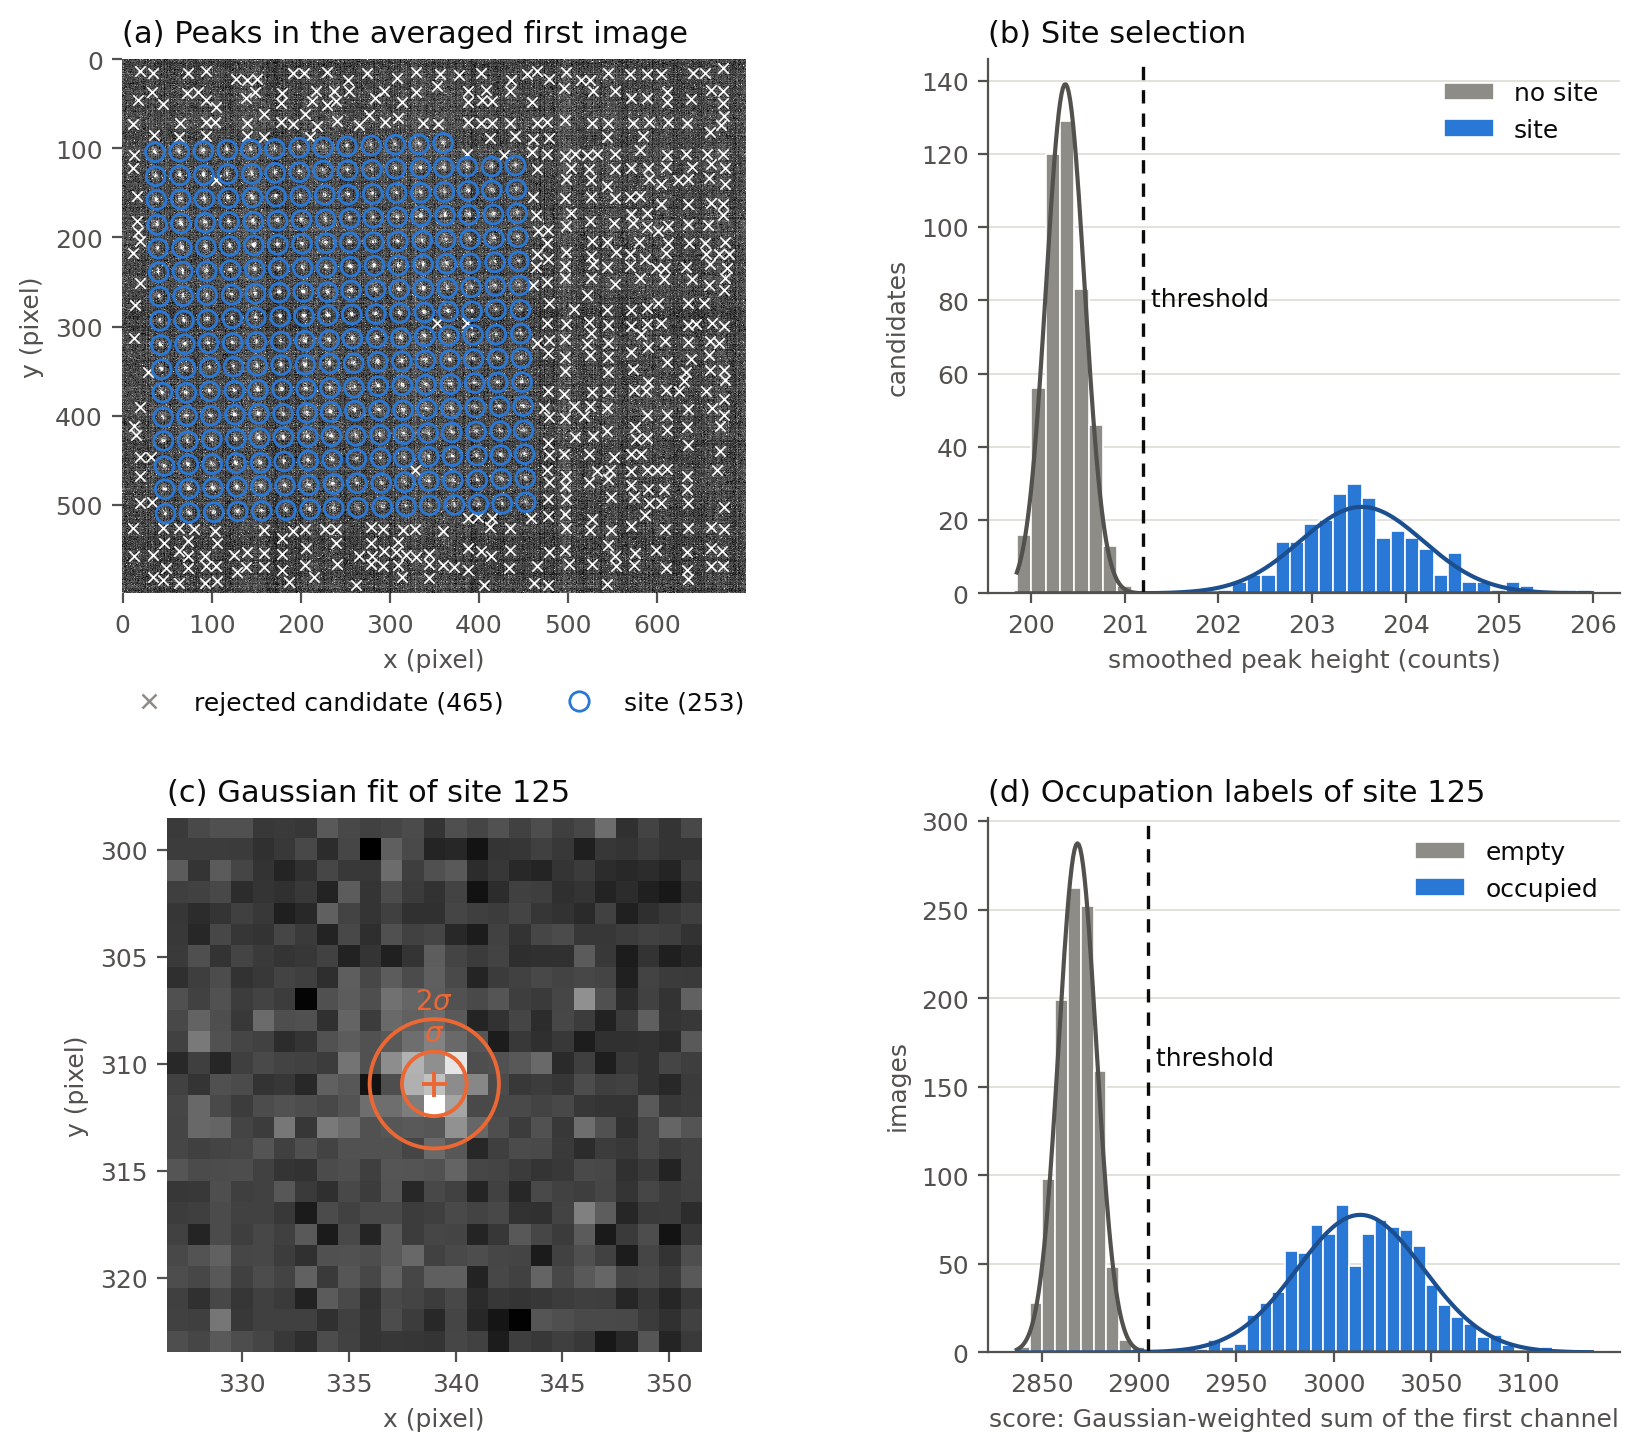
\includegraphics[width=0.95\textwidth]{experimental_labeling.png}
    \caption[Labeling workflow of the experimental dataset.]{Labeling workflow of the experimental dataset. (a) Local maxima of the smoothed average of the first channel: rejected candidates (crosses) and retained sites (circles). (b) Site selection: Peaks above the threshold are sites. (c) Circular Gaussian fit of one site (site 125) with the radii $\sigma$ and $2\sigma$. (d) Occupation labels of site 125: Scores above the threshold are labeled occupied, the others empty.}
    \label{fig:experimental-labeling}
\end{figure}


\subsubsection{Split and Normalization}

Each dataset is randomly split into \SI{60}{\percent} training, \SI{20}{\percent} validation and \SI{20}{\percent} test images, as in the experimental work~\cite{phuttitarn2023}. This results in 3601, 1200, and 1201 images for each simulated dataset, and 1214, 404, and 406 images for the experimental dataset.
The split is applied to whole images, so all sites of a given image always belong to the same subset.
Training images are used to fit the models and to compute the mean $\mu$ and the range $I_{\max}-I_{\min}$ for normalization, defined as $I' = (I-\mu)/(I_{\max}-I_{\min})$.
Validation images are used to select the checkpoint, window size, and threshold. All reported results are computed using the test images.

\subsection{Baseline Detectors}

The MF site and MF array models of Kent et al.~\cite{kent2025} and the CNN site of Phuttitarn et al.~\cite{phuttitarn2023} are used as baselines. The square and Gaussian threshold filters and the projection-based state reconstruction of Wei~\cite{wei2023}, which Winklmann et al.\ include in their comparison~\cite{winklmann2024}, serve as classical references. The matched filters are trained as in the original work: the window size $s$ is chosen on the validation images, the weights are learned by linear least squares, and the threshold is set to the value that maximizes the validation fidelity.


The CNN site has the following architecture: three $3\times3$ convolutional layers with 32, 64, and 128 filters, followed by two fully connected layers, for a total of 355\,202 trainable parameters. One model is trained per exposure time across the crops of all nine sites, using the Adam optimizer with a learning rate of $10^{-4}$, a batch size of 64, and cross-entropy loss. All hyperparameters are listed in Appendix~\ref{app:training}.


As in Kent et al.~\cite{kent2025} and Phuttitarn et al.~\cite{phuttitarn2023}, the infidelity $1-\mathcal{F}$ is defined as
\begin{equation}
 \mathcal{F} = 1 - \frac{P(B'|D) + P(D'|B)}{2},
\label{eq:fidelity}
\end{equation}
where $P(B'|D)$ is the probability that a dark site is classified as bright and $P(D'|B)$ is the probability that a bright site is classified as dark. It is evaluated on the test images for each exposure time at each site, then averaged across the nine sites.

\begin{figure}[tbp]
    \centering
    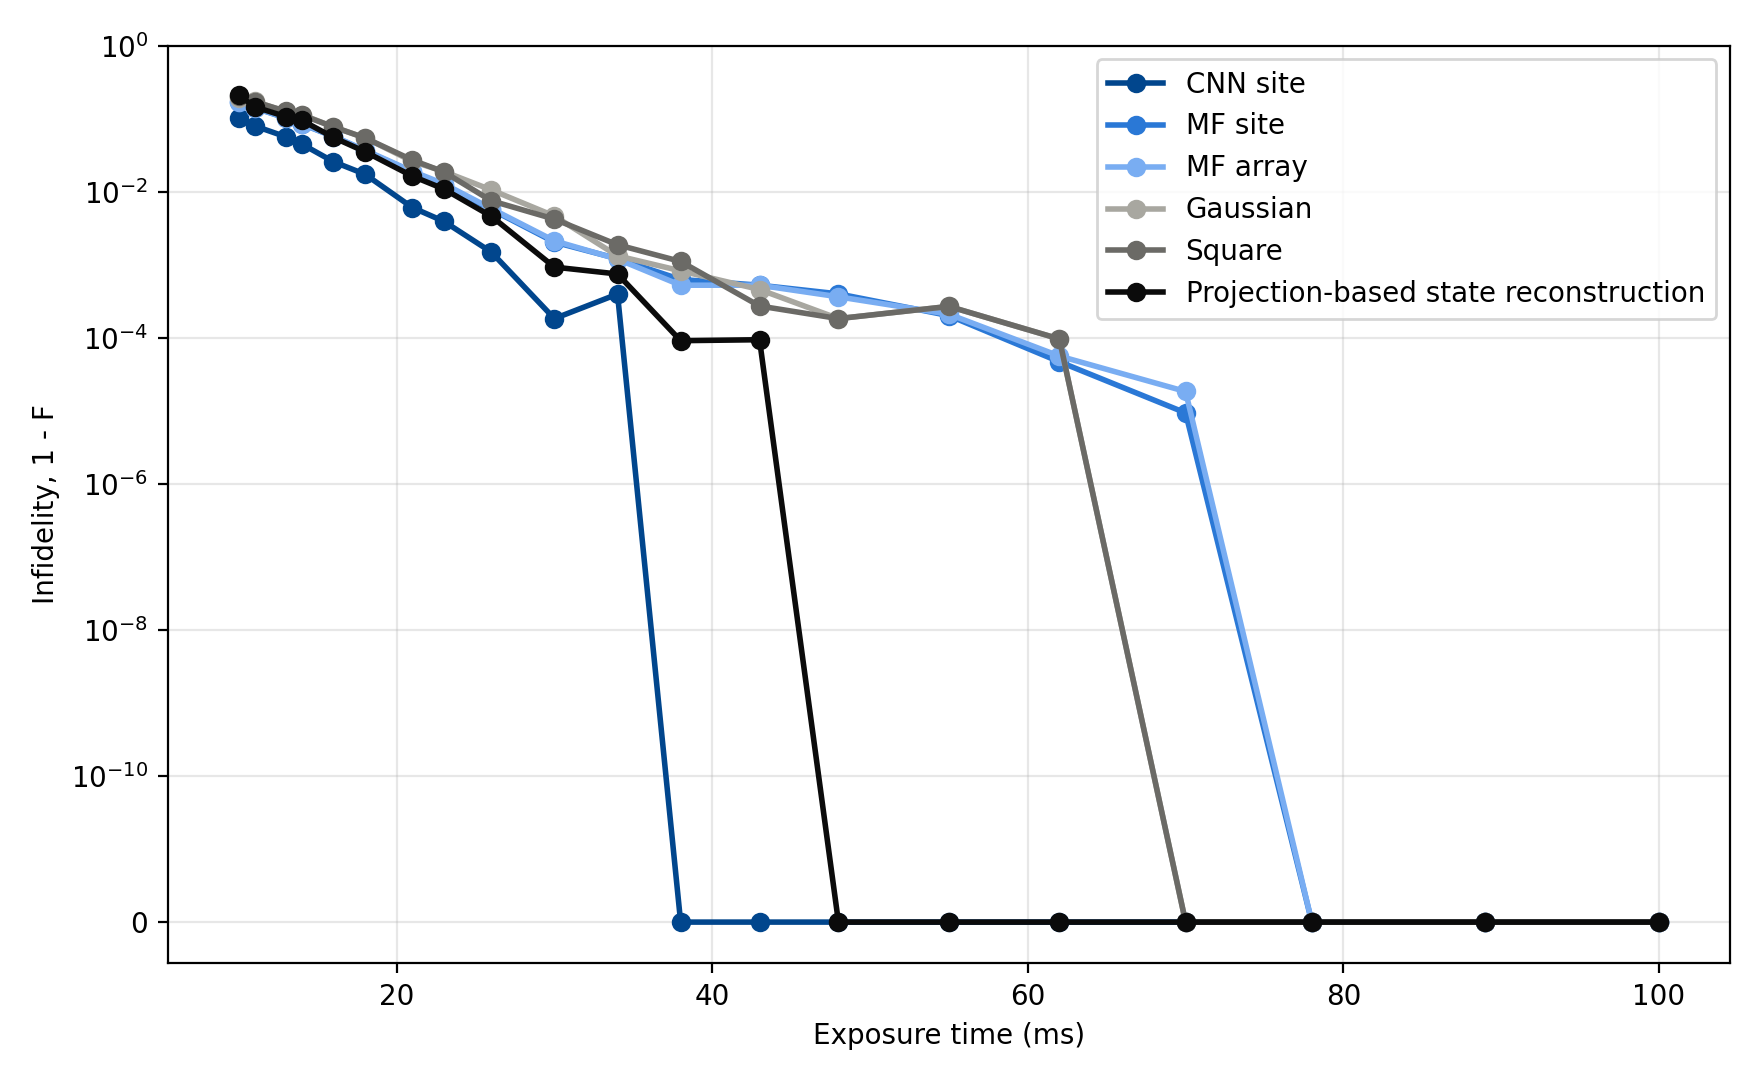
\includegraphics[width=0.85\textwidth]{fidelity_vs_exposure.png}
    \caption{Baselines infidelity versus exposure time.}
    \label{fig:baselines}
\end{figure}

\Cref{fig:baselines} shows the infidelity of all methods. It decreases with exposure time, but the CNN site is the most accurate, outperforming MF site and MF array in 17 of 20 exposure times. The remaining three are long exposures, for which both have no errors on the test set. Compared with MF site and MF array, the CNN site lowers the infidelity by about \SI{40}{\percent} at \SI{10}{\milli\second}, by about \SI{67}{\percent} at \SI{21}{\milli\second} and by about \SI{91}{\percent} at \SI{30}{\milli\second}. Its infidelity stays below $10^{-2}$ from \SI{21}{\milli\second} on, whereas the matched filters need \SI{26}{\milli\second}. The projection-based state reconstruction is the best among the other methods at medium exposures, reaching zero error at \SI{48}{\milli\second}, while the square and Gaussian filters reach zero error at \SI{70}{\milli\second}. In the experimental data of Kent et al.\ the matched filters reach about the same fidelity as the CNN site~\cite{kent2025}, whereas in the simulation, the CNN site is clearly better.

The CNN site is more accurate than the other methods, but its 355\,202 parameters and the wide convolutional layers do not allow the FPGA to meet the desired latency of a few microseconds. The next section, therefore, details how the CNN is reduced by about \SI{99}{\percent} while maintaining the same fidelity.

\newpage
\section{Network Design}\label{sec:network}

The CNN site in \cref{sec:simbase} is accurate, but \SI{74}{\percent} of its parameters reside in the first fully connected layer, which is a poor match for an FPGA. This research proposes TinyCNN, which preserves the CNN site architecture while drastically reducing network parameters and improving hardware friendliness (\cref{fig:tinycnn}).

\begin{figure}[H]
    \centering
    \resizebox{\textwidth}{!}{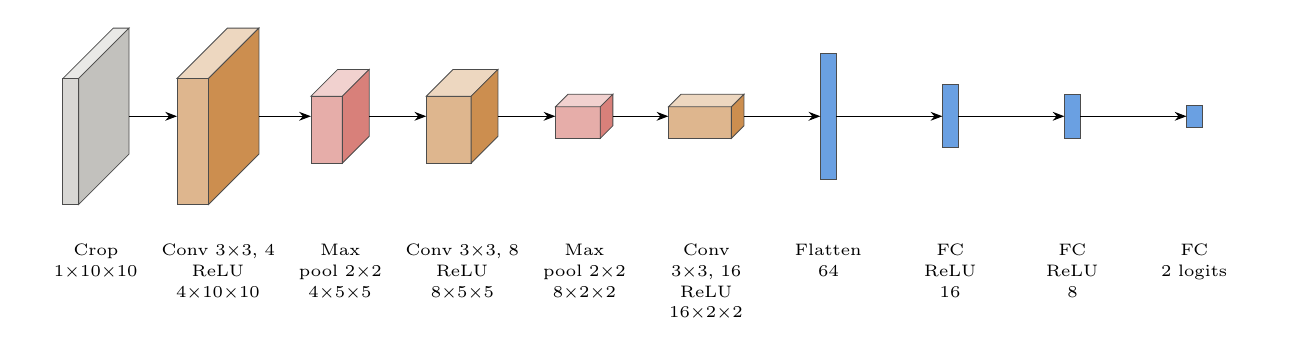
\begin{tikzpicture}[x=1cm, y=1cm]
    \fmap{0}{0.2}{1.6}{cInput}{in}{Crop}{$1{\times}10{\times}10$}{-1.5}
    \fmap{1.55}{0.4}{1.6}{cConv}{c1}{Conv $3{\times}3$, 4\\ReLU}{$4{\times}10{\times}10$}{-1.5}
    \fmap{3.1}{0.4}{0.85}{cPool}{p1}{Max pool $2{\times}2$}{$4{\times}5{\times}5$}{-1.5}
    \fmap{4.65}{0.57}{0.85}{cConv}{c2}{Conv $3{\times}3$, 8\\ReLU}{$8{\times}5{\times}5$}{-1.5}
    \fmap{6.2}{0.57}{0.4}{cPool}{p2}{Max pool $2{\times}2$}{$8{\times}2{\times}2$}{-1.5}
    \fmap{7.75}{0.8}{0.4}{cConv}{c3}{Conv $3{\times}3$, 16\\ReLU}{$16{\times}2{\times}2$}{-1.5}
    \fcbar{9.3}{64}{cFc}{fl}{Flatten}{64}{-1.5}
    \fcbar{10.85}{16}{cFc}{f1}{FC\\ReLU}{16}{-1.5}
    \fcbar{12.4}{8}{cFc}{f2}{FC\\ReLU}{8}{-1.5}
    \fcbar{13.95}{2}{cFc}{f3}{FC}{2 logits}{-1.5}
    \draw[flow] (in-r) -- (c1-l);
    \draw[flow] (c1-r) -- (p1-l);
    \draw[flow] (p1-r) -- (c2-l);
    \draw[flow] (c2-r) -- (p2-l);
    \draw[flow] (p2-r) -- (c3-l);
    \draw[flow] (c3-r) -- (fl-l);
    \draw[flow] (fl-r) -- (f1-l);
    \draw[flow] (f1-r) -- (f2-l);
    \draw[flow] (f2-r) -- (f3-l);
\end{tikzpicture}
}
    \caption[The TinyCNN without neighbor injection.]{The TinyCNN without neighbor injection. The sizes below the blocks are channels $\times$ height $\times$ width.}
    \label{fig:tinycnn}
\end{figure}

\subsection{Convolutional layers} All three convolutions use a $3\times3$ kernel with stride 1 and padding 1. With this padding, the height and width of the feature map stay the same as at the input, so the convolutions do not shrink the $10\times10$ crop and no border pixels are lost. The resolution is reduced only by max pooling with a $2\times2$ window after the first two convolutions, from $10\times10$ to $5\times5$ and to $2\times2$. Max pooling and the rectified linear unit (ReLU) do not require multiplications, so both are cheap on hardware and only require comparisons. The channel count is also reduced from 32, 64, and 128 to 4, 8, and 16. After the last convolution, the flattened feature vector has 64 values instead of 2048.

\subsection{Fully connected layers} The large first fully connected layer of the CNN site is replaced by a small stack of hidden layers with 16 and 8 neurons. Using the smaller flattened vector reduces the classifier from 262\,530 to 1194 parameters. The two outputs are logits. A site is classified as occupied if the second logit is larger than the first, which is equivalent to choosing the larger softmax probability, so no softmax is needed at inference.

\subsection{Neighbor injection} The MF array of Kent et al.\ appends the mean pixel value of the region surrounding each neighboring site to the site's feature vector~\cite{kent2025}. This approach is implemented in the TinyCNN.
For each site, the mean pixel value is computed across the crops of its eight neighbors in the array, and these eight values are provided as input to the network. In a second variant, the plain mean is replaced by a Gaussian-weighted mean, $\sum G\,I / \sum G$ with $G(x,y) = \exp(-(x^2+y^2)/(2\sigma^2))$ centered on the neighbor, so that the pixels at its center count most. Here, $\sigma$ is the width of the point-spread function, modeled as a Gaussian fitted to the average training image. If a neighbor lies outside the array, it is replaced by the noise floor, defined as the mean value of an empty site, computed in the same way as the neighbor values, as shown for a corner site in Appendix~\ref{app:neighbors}.
All values are scaled by a constant derived from the training images. The position of this injection is critical. Appending the eight values to the flattened vector would dilute them among the 72 input features. Appending them immediately before the output logits would prevent them from being processed by a hidden layer. To address this, the first fully connected layer is reduced to eight features, which are then concatenated with the eight neighbor values. The resulting network head is illustrated in \cref{fig:tinycnn-injection}. The following variants are considered: TinyCNN, TinyCNN with neighbors, and TinyCNN with Gaussian neighbors.

\begin{figure}[H]
    \centering
    \resizebox{0.75\textwidth}{!}{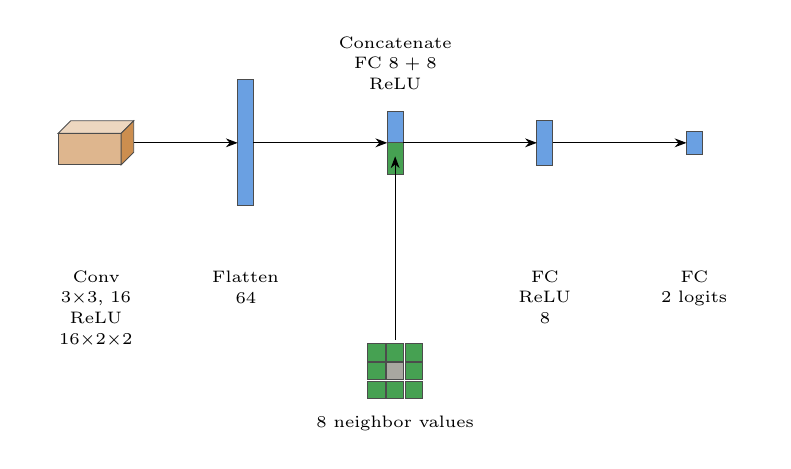
\begin{tikzpicture}[x=1cm, y=1cm]
    \fmap{0}{0.8}{0.4}{cConv}{c3}{Conv $3{\times}3$, 16\\ReLU}{$16{\times}2{\times}2$}{-1.5}
    \fcbar{1.9}{64}{cFc}{fl}{Flatten}{64}{-1.5}

    \pgfmathsetmacro{\bh}{0.2*sqrt(16)}
    \draw[fill=cFc!70, draw=black!70, line width=0.3pt] (3.8-0.1,0) rectangle (3.8+0.1,\bh/2);
    \draw[fill=cNeighbor!85, draw=black!70, line width=0.3pt] (3.8-0.1,-\bh/2) rectangle (3.8+0.1,0);
    \coordinate (cat-l) at (3.8-0.1,0);
    \coordinate (cat-r) at (3.8+0.1,0);
    \node[anchor=south, align=center, text width=1.5cm, font=\fontsize{6.5}{7.5}\selectfont] at (3.8,0.55) {Concatenate\\FC $8+8$\\ReLU};

    \fcbar{5.7}{8}{cFc}{f2}{FC\\ReLU}{8}{-1.5}
    \fcbar{7.6}{2}{cFc}{f3}{FC}{2 logits}{-1.5}

    \foreach \row in {0,1,2}{
        \foreach \col in {0,1,2}{
            \pgfmathsetmacro{\px}{3.8+(\col-1)*0.24}
            \pgfmathsetmacro{\py}{-2.9-(\row-1)*0.24}
            \ifnum\row=1
                \ifnum\col=1
                    \draw[fill=cInput, draw=black!70, line width=0.3pt] (\px-0.11,\py-0.11) rectangle (\px+0.11,\py+0.11);
                \else
                    \draw[fill=cNeighbor!85, draw=black!70, line width=0.3pt] (\px-0.11,\py-0.11) rectangle (\px+0.11,\py+0.11);
                \fi
            \else
                \draw[fill=cNeighbor!85, draw=black!70, line width=0.3pt] (\px-0.11,\py-0.11) rectangle (\px+0.11,\py+0.11);
            \fi
        }
    }
    \node[anchor=north, align=center, text width=2.6cm, font=\fontsize{6.5}{7.5}\selectfont] at (3.8,-3.35) {8 neighbor values};
    \draw[flow] (3.8,-2.5) -- (3.8,-\bh/2-0.03);

    \draw[flow] (c3-r) -- (fl-l);
    \draw[flow] (fl-r) -- (cat-l);
    \draw[flow] (cat-r) -- (f2-l);
    \draw[flow] (f2-r) -- (f3-l);
\end{tikzpicture}
}
    \caption[Head of the TinyCNN with neighbor injection, starting at the last convolution.]{Head of the TinyCNN with neighbor injection, starting at the last convolution. The layers before it are the same as in \cref{fig:tinycnn}. The 8 features of the site (blue) are concatenated with the 8 neighbor values (green) before the second hidden layer.}
    \label{fig:tinycnn-injection}
\end{figure}

\subsection{Size and training} \Cref{tab:size} compares the size of the networks. The TinyCNN with injection has about \SI{99}{\percent} fewer parameters and about \SI{99}{\percent} fewer multiply-accumulate operations than the CNN site. The TinyCNN is trained with the same optimizer and loss as the CNN site, but with its own hyperparameters, including an 800-epoch maximum budget with early stopping. All values are listed in Appendix~\ref{app:training}.

\begin{table}[tbp]
    \centering
    \caption{Parameters and multiply-accumulate operations (MACs) per site.}
    \label{tab:size}
    \begin{tabular}{@{}lrr@{}}
        \toprule
        Network & Parameters & MACs \\
        \midrule
        CNN site & 355\,202 & 2\,124\,032 \\
        TinyCNN & 2698 & 16\,576 \\
        TinyCNN with neighbors & 2178 & 16\,064 \\
        \bottomrule
    \end{tabular}
\end{table}

\newpage
\section{Deep Learning Results}\label{sec:dlresults}

The TinyCNN variants described in \cref{sec:network} are compared with the CNN site by evaluating the difference in their fidelities, expressed in percentage points (p.p.), where $\Delta \mathcal{F} = \mathcal{F}_{\text{TinyCNN}} - \mathcal{F}_{\text{CNN site}}$ and $\mathcal{F}$ denotes the fidelity defined in \cref{eq:fidelity}. A positive value indicates an improvement, corresponding to fewer errors than the CNN site, while a negative value indicates a higher error rate. One percentage point represents one percent of the test decisions being correct or incorrect. The simulated test set has 10\,809 decisions (1201 images with 9 sites each), so 1 p.p. corresponds to approximately 108 decisions, and a single incorrect decision represents \num{0.0093} p.p. The experimental test set contains 102\,718 decisions (406 images with 253 sites each), so 1 p.p. is approximately 1027 decisions, and one incorrect decision corresponds to \num{0.0010} p.p. These values are indicated in the figure legends.

\subsection{Simulated Data}

\begin{figure}[H]
    \centering
    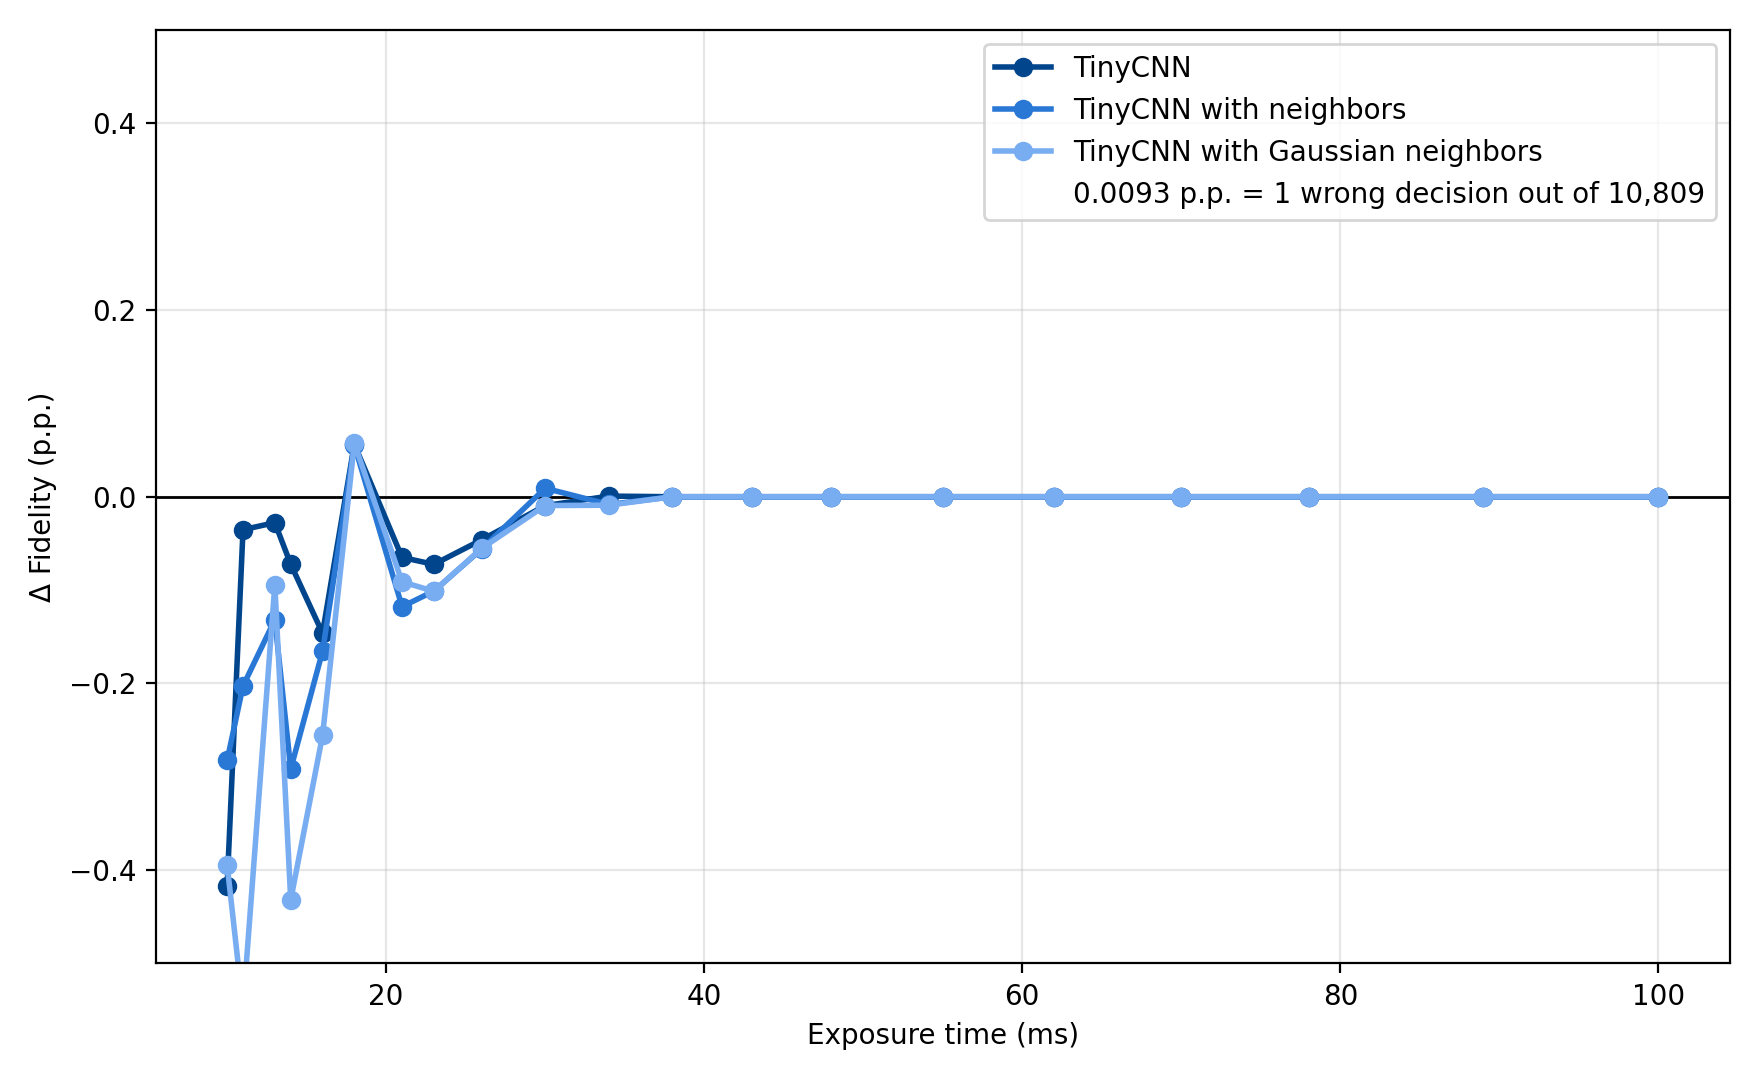
\includegraphics[width=0.85\textwidth]{fidelity_delta_from_cnn_site.png}
    \caption[Fidelity difference of the TinyCNN variants to the CNN site on the simulated data.]{Fidelity difference of the TinyCNN variants to the CNN site on the simulated data. Positive values are an improvement over the CNN site.}
    \label{fig:delta-sim}
\end{figure}

\Cref{fig:delta-sim} presents $\Delta \mathcal{F}$ as a function of exposure time. From \SI{38}{\milli\second} onward, $\Delta \mathcal{F}$ is zero for all variants. From \SI{30}{\milli\second} onward, the difference is at most one incorrect decision. At shorter exposure times, the differences remain small and fluctuate in sign. Up to \SI{26}{\milli\second}, the TinyCNN variants have a slightly higher error rate than the CNN site, averaging \num{0.09}\,p.p.\ for TinyCNN, \num{0.14}\,p.p.\ with neighbors, and \num{0.21}\,p.p.\ with Gaussian neighbors, with a maximum of \num{0.55}\,p.p., corresponding to approximately 59 decisions. Despite having approximately \SI{99}{\percent} fewer parameters than the CNN site, TinyCNN maintains the fidelity within a few tenths of a percentage point.

\subsection{Experimental Data and Model Selection}

\begin{figure}[H]
    \centering
    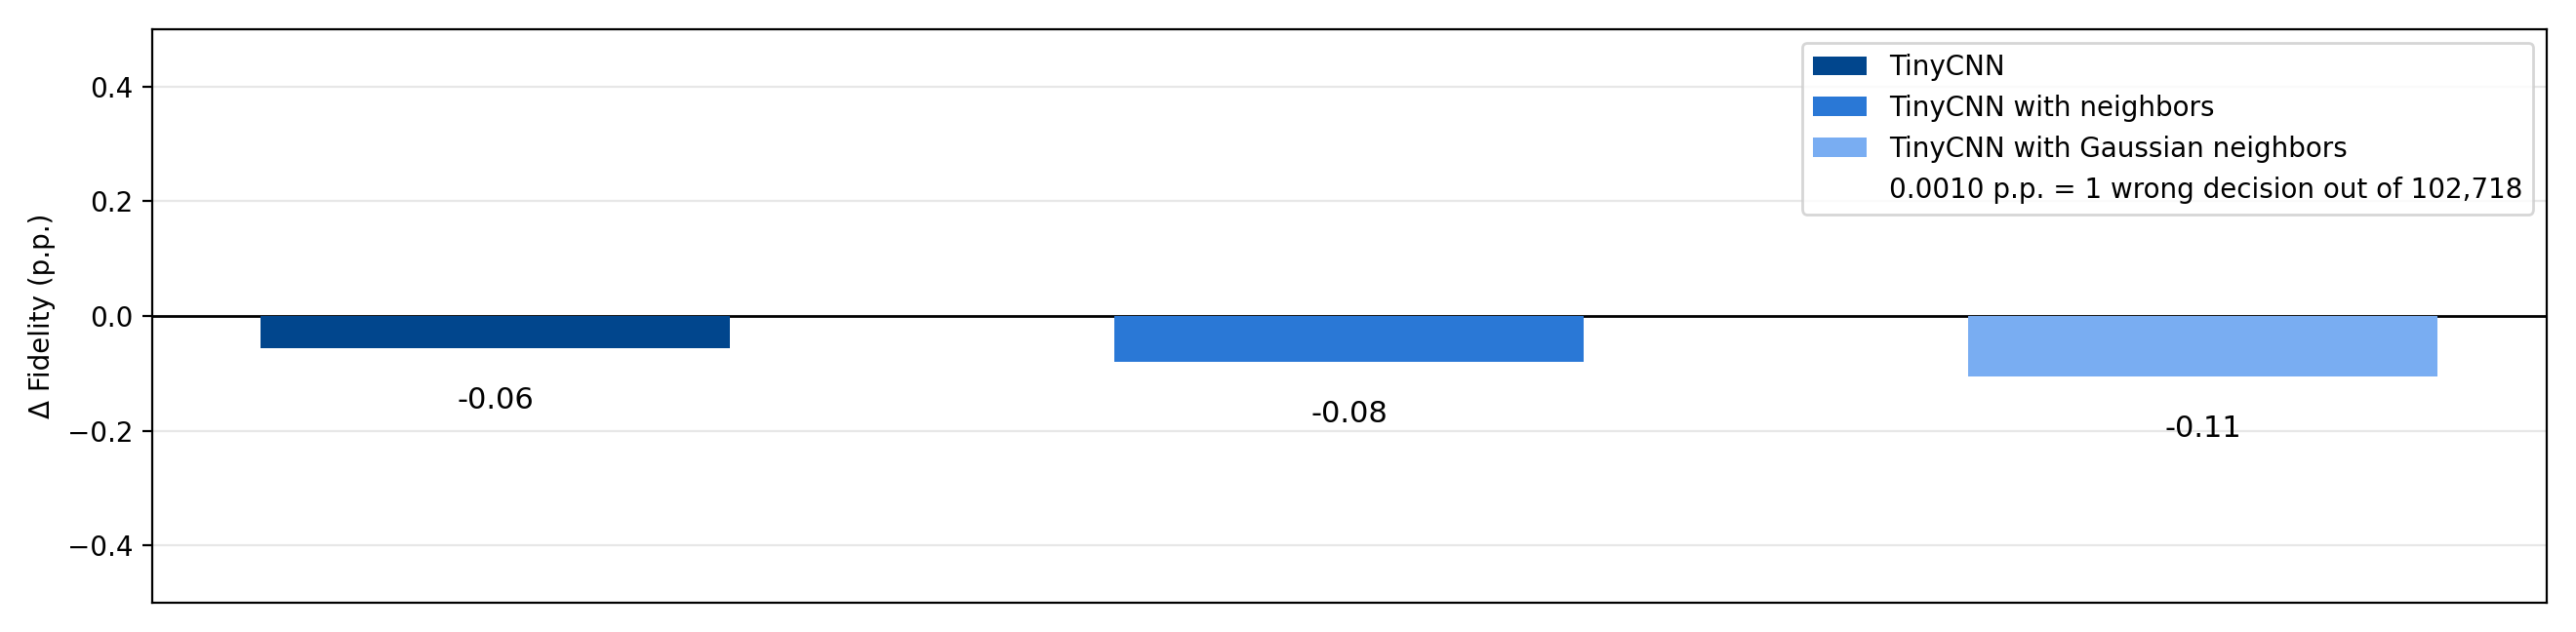
\includegraphics[width=1\textwidth]{real_dataset_vs_cnn_site.png}
    \caption[Fidelity difference of the TinyCNN variants to the CNN site on the experimental data.]{Fidelity difference of the TinyCNN variants to the CNN site on the experimental data. Positive values are an improvement over the CNN site.}
    \label{fig:delta-real}
\end{figure}

The experimental dataset consists of 2024 images of $600\times700$ pixels with 253 sites. In comparison with the simulation, the sites are farther apart, about 27 instead of 7 pixels, and the point-spread function is wider, with a width of 2.6 instead of 0.9 pixels. Therefore, the models are trained on $20\times20$ pixel crops instead of $10\times10$ pixel crops.
\Cref{fig:delta-real} shows that all three TinyCNN variants have a lower fidelity than the CNN site on the experimental data: by \num{0.06}\,p.p.\ for the TinyCNN, \num{0.08}\,p.p.\ with neighbors, and \num{0.11}\,p.p.\ with Gaussian neighbors. The differences between the variants are small, 21 to 45 errors out of about 1700, which is comparable to the fluctuation of an error count of this size, so the ordering may be noise.

\medskip
No variant is clearly best. On the experimental data, the TinyCNN without neighbors is nominally the closest to the CNN site, and in the simulation it is the best of the three at 8 of the 11 exposure times where the variants differ, against 2 for the neighbors and 1 for the Gaussian neighbors. The neighbor information therefore gives no measurable advantage at the spacings of these datasets. The TinyCNN with neighbors is used for the FPGA implementation because it has fewer parameters than the TinyCNN without neighbors, and because the mean of a crop requires only additions, whereas the Gaussian-weighted mean requires a multiplication for each pixel. The variants share the loss, optimizer, and data split procedure; the maximum training budget and early stopping settings are listed in Appendix~\ref{app:training}.
\newpage
\section{Post-Training Quantization}\label{sec:quant}

The trained network undergoes post-training quantization through a three-step process. First, the network tensors are profiled to determine their ranges. Second, sensitivity analysis assesses the extent to which each network layer can be narrowed. Third, width optimization identifies the most cost-effective set of widths for all components collectively. The quantized network is subsequently executed as an integer model in NumPy, and its outputs are compared with those of the float32 network on the test images. Following the methodology of Su et al.~\cite{su2026}, who report classification accuracy within \SI{0.05}{\percent} of the floating-point model, the objective is to achieve a difference in infidelity of no more than \SI{0.05}{p.p.} relative to the float32 model.

\subsection{Profiling} The float32 network is run on the validation images, and the value range of each tensor is recorded. This includes weights, biases, layer outputs, and inputs.
Each tensor is assigned a fixed-point format characterized by $W$ total bits, where $I$ bits represent the integer portion, including the sign. Values are rounded to the nearest representable number and saturate at the format limits.
The integer bits $I$ and fractional bits $F$ for each tensor follow the rules in \cref{tab:profile-rules}, with $W = I + F$.


\begin{table}[H]
  \centering
  \caption{Profiling rules of each tensor.}
  \label{tab:profile-rules}
  \begin{tabular}{@{}lll@{}}
    \toprule
    Tensor & Integer bits $I$ & Fractional bits $F$ \\
        \midrule
            Weights & $I = \lfloor\log_2 \max|x|\rfloor + 2$ & $F_w = W_w - I_w$, with $W_w \le 18$ \\
            Inputs and layer outputs & $I = \lfloor \log_2 \max(|x_{0.1}|,\,|x_{99.9}|) \rfloor + 2$ & $F_a = W_a - I_a$, with $W_a \le 27$ \\
            Accumulators & $\lfloor \log_2 \sum_i |w_{c,i}| \rfloor + I_{\mathrm{in}} + 1$ & $F_{\mathrm{acc}} = F_w + F_{\mathrm{in}}$ \\
            Biases & $I = \lfloor\log_2 \max|x|\rfloor + 2$ & $F_{\mathrm{bias}} = F_{\mathrm{acc}}$ \\
        \bottomrule
    \end{tabular}
\end{table}


For inputs and layer outputs, $x_{99.9}$ and $x_{0.1}$ denote the 99.9th and 0.1th percentiles of the tensor.
For weights and activations, $W_w$ and $W_a$ represent their respective total bit widths, and $I_w$ and $I_a$ their respective integer bits.
For accumulators, $c$ refers to the output channel with the largest sum of absolute weights $w_{c,i}$, while $I_{\mathrm{in}}$ and $F_{\mathrm{in}}$ represent the integer and fractional bits of the layer input, respectively. The 18- and 27-bit limits correspond to the operand widths of the multiplier in a DSP48E2 block of the Alveo U55C. In the following steps, the ratio is preserved such that $W_a = \mathrm{round}(27/18\,W_w)$.
This profile is intentionally broad and serves as the initial configuration for the following sensitivity analysis.

\subsection{Sensitivity} To determine the minimum feasible width for each network component, the network is partitioned into six blocks: the input with the first convolution, the second convolution, the third convolution, the first fully connected layer, the neighbor values with the second fully connected layer, and the output layer. Each convolution block includes its activation and, where applicable, its pooling. The weight width $W_w$ of one block at a time is swept from 2 to 20 bits, while the remaining blocks keep their profiled widths. The integer bits $I_w$ remain at their profiled values, resulting in changes only to the fractional bits $F_w = W_w - I_w$. In the block under evaluation, the activation width is set according to $W_a = \mathrm{round}(27/18\,W_w)$, with fixed integer bits $I_a$ and $F_a = W_a - I_a$. Accumulators and biases are configured according to the rules in \cref{tab:profile-rules}. Each configuration is evaluated by running the integer model on the complete test set. The primary metric is the change in infidelity relative to the float32 network, $\Delta\mathrm{Infidelity} = (1 - \mathcal{F}_{\mathrm{fixed}}) - (1 - \mathcal{F}_{\mathrm{float}})$, expressed in percentage points, where $\mathcal{F}$ is defined in \cref{eq:fidelity}.

\subsection{Width optimization} Width optimization aims to identify the lowest-cost weight widths $W_w$ for all six blocks simultaneously, ensuring that $|\Delta\mathrm{Infidelity}| \le 0.05$ percentage points. This threshold corresponds to approximately five decisions out of the 10\,809 in the simulated test set. Activation widths are determined by $W_a = \mathrm{round}(27/18\,W_w)$. The cost metric serves as a proxy for multiplier area and is calculated as the sum of the number of multiplications across all blocks, multiplied by $W_w$ and $W_a$. The search begins at the narrowest width for each block that individually satisfies the sensitivity analysis band. Because blocks are evaluated independently, their combination often falls outside the acceptable band. During the repair phase, the block with the highest sensitivity at its current width is incrementally widened by one bit until the combined configuration meets the band criterion. In the descent phase, one bit is removed from the block where this change saves the most cost. The first reduction that maintains the configuration within the band is accepted, and this process is repeated until no further single-bit reductions are feasible. This approach yields a local minimum with respect to single-bit adjustments. The weight width is capped at 18 bits, all evaluated combinations are cached, and the total number of evaluations is limited to 150. The optimization hyperparameters are detailed in Appendix~\ref{app:optimizer}.

With the widths in \cref{tab:widths}, the quantized network is run once more as an integer model on the test set. The difference in infidelity to the float32 network is \SI{0.04}{p.p.}, which is within the target of \SI{0.05}{p.p.} and corresponds to about four decisions of the 10\,809. The integer model also serves as the bit-accurate reference for the hardware. The widths are therefore fixed, and the network is implemented in hardware, as described in \cref{sec:fpga}.

\begin{table}[H]
    \centering
    \caption{Optimization results for the TinyCNN with neighbors at \SI{10}{\milli\second} on the simulated data.}
    \label{tab:widths}
    \begin{tabular}{@{}lcccccc@{}}
        \toprule
        Block & $W_w$ & $I_w$ & $W_a$ & $I_a$ & $W_{\mathrm{acc}}$ & $I_{\mathrm{acc}}$ \\
        \midrule
        Input and first convolution & 5 & 1 & 8 & 1 & 14 & 3 \\
        Second convolution & 6 & 2 & 9 & 2 & 16 & 5 \\
        Third convolution & 4 & 1 & 6 & 3 & 17 & 7 \\
        First fully connected layer & 6 & 2 & 9 & 5 & 15 & 8 \\
        Neighbors and second fully connected layer & 6 & 1 & 9 & 5 & 16 & 7 \\
        Output layer & 5 & 1 & 8 & 5 & 15 & 7 \\
        \bottomrule
    \end{tabular}
\end{table}
\newpage
\section{FPGA Implementation}\label{sec:fpga}

\subsection{Hardware overview}
The hardware consists of a preprocessor and a CNN core (\cref{fig:hardware-overview}). The preprocessor prepares the site crops and their neighbor values. Within the CNN core, an activation buffer stores the input crop and intermediate layer outputs. Input routing modules select and distribute the activations to an array of 100 multiply-accumulate (MAC) units. Weight and bias handlers supply the corresponding parameters from separate read-only memories (ROMs). The MAC results pass through requantization and, after the first two convolutional layers, max pooling. The layer output module arranges the results for the next layer or supplies the final two logits. A controller coordinates the memory reads, MAC operations, and progression through the six layers. Pipeline registers between these stages shorten the critical paths so that the design can run at a higher clock frequency.
\begin{sidewaysfigure}
    \centering
    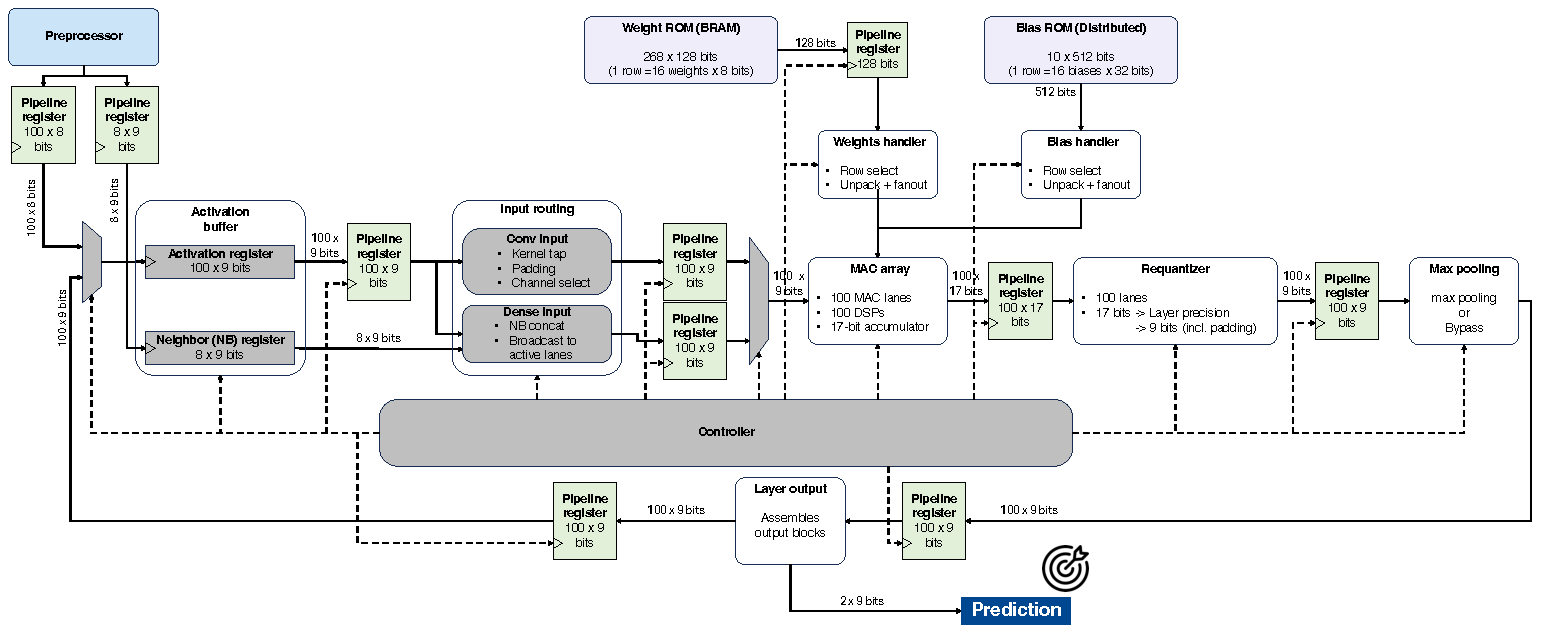
\includegraphics[width=\textheight]{hardware_overview_cropped.pdf}
    \caption{Hardware overview of the CNN core.}
    \label{fig:hardware-overview}
\end{sidewaysfigure}

\subsection{Preprocessing}
The preprocessor (\cref{fig:preprocessor}) converts a $28\times28$ frame into nine site inputs. Each input consists of a $10\times10$ crop and eight neighbor values. Crop extraction and normalization are performed incrementally as pixels arrive. After processing the entire frame, neighbor values are computed, and the site inputs are sequentially presented to the convolutional neural network (CNN).
\begin{figure}[tbp]
    \centering
    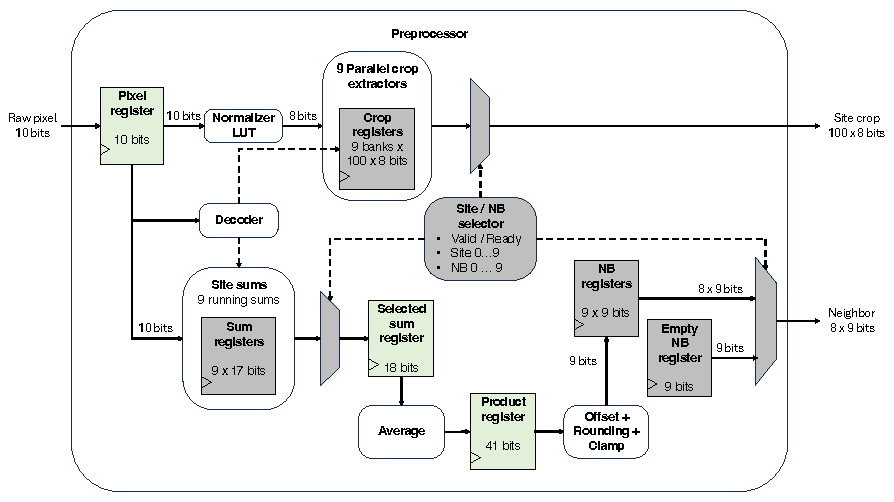
\includegraphics[width=0.95\textwidth]{preprocessing_cropped.pdf}
    \caption{Block diagram of the preprocessor.}
    \label{fig:preprocessor}
\end{figure}

\subsubsection{Pixel input and normalizer}
The input interface receives one unsigned 10-bit pixel per clock cycle when the valid signal is asserted. Pixels are delivered in row-major order, proceeding from left to right and top to bottom. Coordinate counters increment with each accepted pixel. Normalization is performed using the mean and scale parameters stored during training
\[
    p_{\mathrm{norm}} = \frac{p_{\mathrm{raw}}-\mu}{s}.
\]
The result for each valid raw pixel value is calculated before synthesis and stored in the \texttt{Normalizer} lookup table. Each raw pixel selects a signed 8-bit normalized value from this table.
\subsubsection{Crop extractors}
The positions of the nine sites are predetermined, resulting in constant starting coordinates for each crop. Nine parallel coordinate checks identify whether a pixel belongs to a given crop. For each matching crop, the pixel's local coordinates specify its position within the corresponding 100-element crop buffer. Each crop buffer contains 100 normalized 8-bit values, resulting in a total storage of 7200 bits across all nine buffers. Due to overlap between adjacent crops, a single incoming pixel may update multiple crop buffers simultaneously. Pixels that do not belong to any crop are discarded.
\subsubsection{Neighbor processor}
In parallel with crop extraction, nine running sums accumulate the raw pixel values associated with each crop. Each sum requires 17 bits, as the maximum sum of 100 unsigned 10-bit pixels is 102300. These sums are reset at the start of each new frame. Upon completion of pixel processing, each crop sum is converted into a neighbor feature. For a given sum $S_j$, the feature before quantization is defined as
\[
    n_j = \frac{S_j/100-\mu}{s\times s_{\mathrm{nb}}},
\]
Here, $s_{\mathrm{nb}}$ denotes the neighbor feature scale parameter stored during training. Consequently, the feature represents the normalized average brightness of the corresponding crop. The hardware implements division and scaling as a single constant multiplication, followed by subtraction of a constant offset. The multiplier applies the combined scaling, while the offset accounts for the stored mean. The result is rounded to the nearest value, with ties rounded to even, and saturated to the signed 9-bit neighbor format. A shared arithmetic unit sequentially processes the nine sums, and the resulting features are stored for later use across all sites. The selected sum is held in an 18-bit signed register, the 17-bit sum plus a sign bit, and its product with the 23-bit constant multiplier is 41 bits wide.
\subsubsection{Preprocessing controller}
A finite-state machine coordinates preprocessing through four states (\cref{fig:preprocessing-controller} in Appendix~\ref{app:preprocessing-controller}):
\begin{enumerate}
    \item \texttt{IDLE:} Accept incoming pixels, populate the crop buffers, and update the running sums. After pixel processing is complete, a start request begins neighbor conversion.
    \item \texttt{NEIGHBOR\_MULTIPLY:} Multiply the selected crop sum by the constant normalization factor.
    \item \texttt{NEIGHBOR\_FINISH:} Subtract the offset, round and saturate the result, and store the neighbor feature. Repeat the conversion for the next crop until all nine features are available.
    \item \texttt{PRESENT\_SITES:} Supply the selected crop and its eight neighbor features. Hold these values until the ready signal is asserted, then advance to the next site. After the ninth site is accepted, assert completion and return to \texttt{IDLE}.
\end{enumerate}


The output consists of an 800-bit crop vector and a 72-bit neighbor vector. A fixed neighbor index table selects the surrounding site features.

\subsection{Activation buffer}
The activation buffer stores the values required by the current CNN layer. It contains 100 signed 9-bit elements, forming a 900-bit vector. At the start of inference, this vector holds the normalized $10\times10$ site crop. As inference progresses, it is reused to store outputs from intermediate layers.
\subsubsection{Writing and reuse}
A multiplexer selects either the captured site crop or the completed output from the layer output module. The site scheduler first captures the crop and neighbor values in packet registers, then loads them into the CNN storage on the following clock edge.
Once an intermediate layer completes, its assembled output overwrites the previous contents. Values are stored consecutively according to the layout required by the next layer. For convolutional feature maps, spatial positions for each channel are grouped together, while dense layer features occupy the initial elements of the vector. If fewer than 100 elements are needed, the remaining positions are zero-filled. All values use a uniform 9-bit storage width, and values with lower signed precision are sign-extended.
\subsubsection{Reading}
The controller initiates a read operation before the input routing module selects activations for a multiply-accumulate (MAC) operation. The complete 100-element vector is read in parallel on a rising clock edge, accompanied by a valid signal. The input routing module subsequently selects the necessary spatial positions or dense input features. Because the buffer contains a complete vector, no address selection is required.
\subsubsection{Neighbor storage}
Eight signed 9-bit neighbor values are stored in a separate 72-bit register. These values are loaded simultaneously with the site crop and remain unchanged as intermediate layer outputs update the activation vector. The dense input module accesses these neighbor values during the second dense layer, where eight features from the previous layer are combined with the eight neighbor features.

\subsection{Input routing}
The input routing modules select the activations required for each MAC operation from the activation buffer. Separate modules handle convolutional and dense layers. A multiplexer selects the module's output according to the current layer.
\subsubsection{Convolutional input}
The convolutional input module receives the convolution index, input channel index, and kernel tap index from the controller. For each active MAC lane, a fixed spatial mapping selects the pixel corresponding to the current tap of the $3\times3$ kernel. Positions outside the feature map are assigned a value of zero, thereby implementing padding at the image boundaries. Different output channels use the same input pixels but different weights. The selected spatial values are repeated across the lanes assigned to those output channels.
The lane arrangement depends on the layer:
\begin{itemize}
    \item Conv0 processes one output channel with 100 spatial
          positions per block, using all 100 lanes.
    \item Conv1 processes four output channels with 25 spatial
          positions each per block, also using all 100 lanes.
    \item Conv2 processes 16 output channels with four spatial
          positions each, using 64 lanes.
\end{itemize}
Unused lanes in Conv2 are assigned a value of zero. The controller iterates through all input channels and kernel taps, and each MAC unit accumulates the contributions to its designated output. The next output blocks reuse the same routing configuration with a new set of weights.
\subsubsection{Dense input}
The dense input module selects one feature using the input feature index provided by the controller. This feature is broadcast to all active output lanes. Each lane receives a different weight and accumulates the result for one output neuron. The first dense layer selects from the 64 flattened outputs of Conv2 and uses eight output lanes. The second dense layer uses eight output lanes and selects from 16 inputs: eight features from the previous layer and eight neighbor values. Neighbor values are converted to the fixed-point format used by the dense input, with rounding and saturation. The final dense layer selects from 8 features and uses 2 lanes to compute the 2 logits. All inactive lanes are assigned a value of zero. In contrast to the convolutional input module, dense input routing does not require spatial mapping or kernel tap selection.

\subsection{MAC array}
A single array of 100 multiply-accumulate (MAC) units executes all three convolutional and three dense layers. The units operate in parallel, with each active lane computing a single output value (\cref{fig:mac-lane}). The controller reuses the array across output blocks, layers, and sites.
\begin{figure}[H]
    \centering
    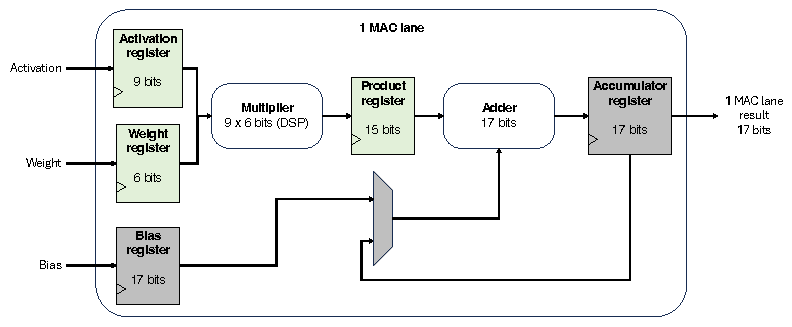
\includegraphics[width=0.8\textwidth]{mac_lane_cropped.pdf}
    \caption{One lane of the MAC array.}
    \label{fig:mac-lane}
\end{figure}

\subsubsection{Arithmetic}
Each lane receives a signed 9-bit activation and a signed 6-bit weight, the widest formats of \cref{tab:widths}. Layers with narrower formats are sign-extended to these widths. Their multiplication produces a signed 15-bit product, which is sign-extended before addition to a 17-bit accumulator. Both multiplication and accumulation are mapped to the FPGA's DSP blocks.
For an output value $y$, the array evaluates
\[
    y = b + \sum_{k=0}^{K-1} a_k w_k,
\]
where $b$ is the bias and $K$ is the number of contributions required for that output. Each valid MAC operation produces one activation-weight pair per lane.
\subsubsection{Bias initialization and accumulation}
During the first contribution to an output block, the controller asserts the bias-load signal and a multiplexer selects the bias as the addend.
\[
    b + a_0 w_0.
\]
For subsequent contributions, the multiplexer selects the previous accumulator value. Thus, bias initialization occurs simultaneously with the first product addition.
\subsubsection{Reuse across layers}
In convolutional layers, each lane accumulates contributions from all input channels and all nine kernel taps. Consequently, Conv0, Conv1, and Conv2 require 9, 36, and 72 products per output value, respectively.
In dense layers, each active lane represents one output neuron and accumulates over the input features. The three dense layers require 64, 16, and 8 products per output neuron,
respectively. Lanes outside the active output group receive zero activations and weights.
After the final contribution to a block, the controller waits until the MAC array has completed its pending operations. The finished accumulator values are then forwarded to the requantization module.

\subsection{Weight ROM and handler}

The weights of all six layers are stored in a synchronous ROM implemented in block RAM. The ROM contains 268 rows of 128 bits. Each row contains 16 signed 8-bit weight slots, with slot zero occupying the least significant bits. The stored weights fit the 6-bit precision used by the MAC array; the handler converts each slot to this width before distribution.

\subsubsection{Weight ROM architecture}
For convolutional layers, one row stores the weights for one input channel and one kernel tap across the output channels of the current block. The weights are shared across all spatial positions within the same output channel.
For dense layers, each row stores the weights connecting a single input feature to all output neurons. The number of rows assigned to each layer is listed in \cref{tab:weight-rows}.

\begin{table}[H]
    \centering
    \caption{Rows of the weight ROM for each layer.}
    \label{tab:weight-rows}
    \begin{tabular}{@{}lrr@{}}
        \toprule
        Layer & First row & Number of rows \\
        \midrule
        Conv0  &   0 & 36 \\
        Conv1  &  36 & 72 \\
        Conv2  & 108 & 72 \\
        Dense0 & 180 & 64 \\
        Dense1 & 244 & 16 \\
        Dense2 & 260 &  8 \\
        \bottomrule
    \end{tabular}
\end{table}

\subsubsection{Address selection}
The handler receives the layer, output block, input channel, and kernel tap indices from the controller and turns them into a row address. The row of a convolutional layer follows from its first row, the output block, the input channel, and the kernel tap, and the row of a dense layer from its first row and the input feature index. The row numbers are fixed constants in the design, so no multiplier is needed.

\subsubsection{Distribution to MAC lanes}
The handler unpacks the selected row and distributes its weights according to the layer's lane arrangement. Conv0 broadcasts a single weight across 100 spatial lanes. Conv1 broadcasts four weights to groups of 25 lanes. Conv2 broadcasts 16 weights to groups of four lanes. For Dense0 and Dense1, eight slots supply one weight to each active output lane. Dense2 uses two slots for its two output neurons. Unused lanes receive zero weights. A read-enable signal requests the ROM row. The row is read on a rising clock edge, and the accompanying valid signal indicates that the weights are available for the MAC operation.

\subsection{Bias ROM and handler}

The biases for all six layers are stored in a compact ROM implemented in distributed memory. This ROM consists of ten 512-bit rows, each divided into 16 signed 32-bit slots, with slot zero occupying the least significant bits. The bias handler retrieves the necessary slots and converts them to the 17-bit accumulator width.

\subsubsection{Bias ROM architecture}
Each convolutional output channel is assigned a single bias shared across all spatial positions, while each dense output neuron receives an individual bias. Consequently, a single ROM row contains all the biases required for a complete output block. The rows are arranged as listed in \cref{tab:bias-rows}.

\begin{table}[H]
    \centering
    \caption{Rows of the bias ROM for each layer.}
    \label{tab:bias-rows}
    \begin{tabular}{@{}lrrr@{}}
        \toprule
        Layer & First row & Number of rows & Used slots per row \\
        \midrule
        Conv0  & 0 & 4 &  1 \\
        Conv1  & 4 & 2 &  4 \\
        Conv2  & 6 & 1 & 16 \\
        Dense0 & 7 & 1 &  8 \\
        Dense1 & 8 & 1 &  8 \\
        Dense2 & 9 & 1 &  2 \\
        \bottomrule
    \end{tabular}
\end{table}

\subsubsection{Address selection}
The handler selects the row from the layer and output block indices supplied by the controller. Convolutional layers advance through their assigned rows as output blocks are processed, whereas each dense layer uses one fixed row.

\subsubsection{Distribution to MAC lanes}
In Conv0, a single bias is broadcast to all 100 spatial lanes. In Conv1, four biases are distributed to groups of 25 lanes each. In Conv2, 16 biases are assigned to groups of four lanes. For dense layers, each active output lane receives an individual bias, while unused lanes are assigned a value of zero. Both the ROM read and the handler's selection logic are combinational. The selected biases are supplied directly to the MAC array, which applies them with the first product addition of each output block. Each bias is therefore added once per output value, regardless of the number of input channels, kernel taps, or dense input features.

\subsection{Requantization}
The requantizer converts the completed MAC accumulators to the activation precision selected for each layer. All 100 lanes are processed in parallel by combinational logic between two pipeline registers. For each layer, a fixed right shift removes the fractional bits that the accumulator has in addition to the output format, that is, the difference $F_{\mathrm{acc}} - F_a$. The result is rounded to the nearest value, with ties rounded to even, and saturated to the representable range. ReLU sets negative values to zero in all layers except the final layer, whose signed outputs form the two logits. The results are sign-extended to the common 9-bit storage width.

\subsection{Max pooling}
Max pooling is performed after the first two convolutional layers. For each output channel, the largest value is selected within each non-overlapping $2\times2$ region, using a stride of two. This operation reduces the spatial dimensions from $10\times10$ to $5\times5$ after Conv0, and from $5\times5$ to $2\times2$ after Conv1. The final row and column of the $5\times5$ feature map are excluded, as they do not constitute complete pooling regions. Conv2 and the dense layers pass their values directly to the layer output module without pooling.

\subsection{Layer output assembly}

The layer output module combines the completed output blocks into the activation layout required by the next layer. The layer and output block indices determine where each block is placed in a 100-element buffer.
Conv0 produces four pooled blocks of 25 values, forming 100 activations. Conv1 produces two pooled blocks of 16 values, forming 32 activations. Conv2 supplies its 64 values in one block. Convolutional values are arranged consecutively by channel, so the Conv2 output also provides the flattened input to the first dense layer.
The first two dense layers each produce eight features, while the final layer produces two logits. Unused buffer elements are filled with zeros.
Once the final block of a layer has been assembled, the module asserts its output-valid signal. The controller then writes the completed vector to the activation buffer for the next layer. For the final layer, the two logits are supplied as the classification result, and the site is classified as occupied if the second logit is larger than the first.

\subsection{Site scheduler}
The site scheduler in \texttt{detector\_core} coordinates preprocessing and the sequential classification of the nine sites. It operates through five states (\cref{fig:site-scheduler} in Appendix~\ref{app:site-scheduler}):
\begin{enumerate}
    \item \texttt{IDLE:} Receive the frame pixels and wait for a start request after frame loading. The start request triggers neighbor feature conversion and advances the scheduler to the next state.
    \item \texttt{WAIT\_SITE:} Wait until the preprocessor presents a valid site packet. Accept the packet and capture its crop, eight neighbor values, and site index in registers. The 100 signed 8-bit crop values are sign-extended to the 9-bit activation width.
    \item \texttt{LOAD\_INPUT:} Load the captured crop into the activation buffer and the captured neighbor values into the separate neighbor register.
    \item \texttt{START\_INFERENCE:} Assert the CNN start signal, then advance to the result-waiting state.
    \item \texttt{WAIT\_RESULT:} Wait for the CNN result valid signal and present the site's logits and decision. Return to \texttt{WAIT\_SITE} for the next site, or assert the completion signal and return to \texttt{IDLE} after site eight.
\end{enumerate}


\subsection{CNN controller}
The controller coordinates the execution of all six layers for one site. A finite-state machine controls the activation and weight reads, MAC operations, and the transfer of completed layer outputs. Counters monitor the current layer, output block, input channel, or feature, and convolutional kernel tap. The controller operates through six distinct states (\cref{fig:cnn-controller} in Appendix~\ref{app:cnn-controller}):
\begin{enumerate}
    \item \texttt{IDLE:} Wait for a start request, then initialize the layer and operation counters.
    \item \texttt{READ\_ACTIVATION:} Request the activation vector from the activation buffer.
    \item \texttt{READ\_WEIGHTS:} Request the weight ROM row corresponding to the current operation.
    \item \texttt{MAC\_STATE:} Wait until both inputs are valid, then issue the MAC operation. The first operation of each output block also loads the biases.
    \item \texttt{EMIT\_BLOCK:} After the final contribution, wait until the MAC array finishes its pending operations, then release the completed accumulators for postprocessing.
    \item \texttt{WAIT\_LAYER\_OUTPUT:} After the final output block, wait for the layer output module to finish assembling the complete layer.
\end{enumerate}

Within convolutional layers, the controller iterates through nine kernel taps for each input channel. In dense layers, it processes input features in sequence. Completing an output block, the controller initiates the next block if further outputs are necessary. Upon finishing an intermediate layer, the controller enables writing to the activation buffer and proceeds to the next layer. After the final dense layer, it asserts the result valid and completion signals, then returns to the idle state.

\newpage
\section{Implementation Results}\label{sec:results}

\subsection{Target and setup}

The design is implemented and deployed on the Alveo U55C accelerator card, which features the Virtex UltraScale+ High Bandwidth Memory (HBM) device XCU55C~\cite{amd2026u55c}. Synthesis, placement, and routing are performed using Vivado and Vitis 2024.2, and the design is tested on the card at \SI{400}{\mega\hertz}. Three hardware counters measure preprocessing, CNN inference for a single site, and the complete nine site pipeline from the first input pixel to the final prediction.

\subsection{Latency}\label{sec:hardware-latency}

The preprocessing counter stops when all neighbor features have been prepared, and the first site input is available. The CNN counter measures the interval from the inference start to the valid logits. The complete pipeline counter measures the interval from the first accepted pixel to the last of the nine predictions, including the handoff between preprocessing and inference and between successive sites.

The conversion from cycles to time is
\[
    t\,[\mu\mathrm{s}] = \frac{N_{\mathrm{cycles}}}{f\,[\mathrm{MHz}]}.
\]
The hardware validation uses eight $28\times28$ test frames, each containing nine sites. All 72 pairs of logits and decisions match the fixed-point reference. \Cref{tab:hardware-latency} lists the counter values, which are identical in all eight validation runs.

\begin{table}[H]
    \centering
    \caption{Hardware-counter measurements at 400 MHz.}
    \label{tab:hardware-latency}
    \begin{tabular}{@{}lrr@{}}
        \toprule
        Measurement & Cycles & Latency ($\mu$s) \\
        \midrule
        Preprocessing, all nine sites & \num{802}  & \num{2.0050} \\
        CNN inference, one site       & \num{858}  & \num{2.1450} \\
        Complete pipeline, nine sites & \num{8559} & \num{21.3975} \\
        \bottomrule
    \end{tabular}
\end{table}

Su et al.~\cite{su2026} report a CNN inference latency of \SI{9.85}{\micro\second} at \SI{500}{\mega\hertz}, excluding preprocessing. The corresponding comparison is with the CNN measurement of this work. The two networks use different architectures and input sizes: Su et al.\ use $20\times20$ site patches, whereas the present model uses $10\times10$ crops and eight neighbor features.
The measured CNN latency of \SI{2.145}{\micro\second} is $4.59\times$ shorter than their published latency, corresponding to a \SI{78.2}{\percent} reduction at a \SI{20}{\percent} lower clock frequency.

\subsection{Resource use}\label{sec:hardware-resources}

Table \ref{tab:hardware-resources} compares routed resource usage with Table III of Su et al. \cite{su2026}. The CNN column offers the most direct comparison to their accelerator. In contrast, the detector column also accounts for preprocessing across nine sites, the site scheduler, packet registers, and latency counters. Both columns omit the Advanced eXtensible Interface (AXI) wrapper and the platform shell.

% Source: data/fpga_runs/2026-10-08/single_cnn_400/utilization_hierarchical_routed.rpt;
% alveo_400_single_cnn_20261008; Su et al., Table III, p. 7.
% Percentages for the CNN hierarchy are calculated from the XCU55C capacity:
% 1,303,680 LUTs; 2,607,360 FFs; 9,024 DSPs; 2,016 BRAM tiles.
\begin{table}[H]
    \centering
    \small
    \setlength{\tabcolsep}{5pt}
    \caption[Resource comparison with Su et al.\ (Table III).]{Resource comparison with Su et al.\ (Table III). Percentages refer to each design's own FPGA. The XCU55C provides 1,304K LUTs, 2,607K flip-flops, 9,024 DSPs and 2,016 BRAM tiles~\cite{amd2026u55c}.}
    \label{tab:hardware-resources}
    \begin{tabular}{@{}lrrr@{}}
        \toprule
        & \shortstack{Su et al.\\CNN, ZCU208}
        & \shortstack{This work\\CNN, U55C}
        & \shortstack{This work\\Detector, U55C} \\
        \midrule
        LUTs & \num{26845} (6.31\%) & \num{19714} (1.51\%) & \num{26824} (2.05\%) \\
        Flip-flops & \num{51943} (6.11\%) & \num{8993} (0.34\%) & \num{17694} (0.68\%) \\
        DSPs & \num{800} (18.73\%) & \num{100} (1.11\%) & \num{101} (1.12\%) \\
        BRAM tiles & \num{491} (45.46\%) & \num{1.5} (0.07\%) & \num{1.5} (0.07\%) \\
        \bottomrule
    \end{tabular}
\end{table}

In absolute counts, the CNN core uses \SI{26.6}{\percent} fewer LUTs, \SI{82.7}{\percent} fewer flip-flops, \SI{87.5}{\percent} fewer DSPs and \SI{99.7}{\percent} fewer BRAM tiles than Su et al.'s implementation.
The 100 MAC lanes account for the CNN's 100 DSPs. Preprocessing adds one DSP for neighbor normalization, \num{6967} LUTs, and \num{7608} flip-flops. The remaining detector logic uses 143 LUTs and \num{1093} flip-flops. Consequently, the complete detector uses 101 DSPs and maintains lower absolute counts across all four resource categories compared to the published accelerator, including \SI{0.08}{\percent} fewer LUTs.

\subsection{Timing closure}\label{sec:timing-closure}

At \SI{400}{\mega\hertz}, the clock period is \SI{2.5}{\nano\second}. Timing closure requires shortening the combinational paths between registers and simplifying the logic on critical paths. Registers introduced for timing closure are shown in light green in the figures (\cref{fig:hardware-overview,fig:preprocessor,fig:mac-lane}).

\subsubsection{CNN core}

The activation buffer read and the outputs of the input routing modules are registered, which separates activation selection from MAC arithmetic. Within each MAC lane, pipeline registers separate the activation and weight inputs, the multiplication stage, and the accumulation stage. Three further pipeline registers divide the processing of completed output blocks. The first captures the finished MAC accumulators before requantization, the second the requantized values before max pooling, and the third the pooled values, or the dense layer bypass values, before layer output assembly. Valid signals, together with their layer and output block indices, are delayed together with the data. Between preprocessing and the CNN, the site scheduler also captures the crop and neighbor packet in pipeline registers. The following \texttt{LOAD\_INPUT} state writes this packet into the CNN's activation storage, and \texttt{START\_INFERENCE} starts execution on the next edge. The convolution layer, input channel, and tap indices are also captured alongside the activation buffer read, so input routing uses metadata aligned with the returned data. These registers separate the long selection and control paths without changing the CNN's 858-cycle execution interval, and they are preserved during synthesis through preservation attributes.

\subsubsection{Preprocessing}

An input register separates pixel reception from normalization and crop selection. During neighbor calculation, selecting a crop sum and multiplying it by the normalization constant forms the critical path. To address this, an additional register is inserted between the sum selection multiplexer and the multiplier, ensuring the selected sum is available before multiplication begins. A product register separates multiplication from offset subtraction, rounding, and saturation. Loading the next sum while completing the current neighbor feature maintains the two-state conversion sequence.

\subsubsection{Combinational logic simplification}

Requantization is tailored to the fixed shift and output width specific to each layer. Rounding is performed on the retained bits, while saturation verifies the discarded upper bits for overflow. This approach reduces arithmetic width and eliminates the need for a general variable shift implementation.

Max pooling is restructured to compare the four input values in parallel, rather than propagating intermediate maxima through sequential comparisons. The comparison results directly select the winning value. When precision conversion is necessary, candidate rounding is performed concurrently with the comparisons. These modifications reduce the pooling path length while preserving the numerical outcome.

\subsubsection{Routed timing result}

Vivado's routed static timing analysis verifies that the complete deployed design, including preprocessing, the CNN, AXI interfaces, and the Alveo platform shell, satisfies all timing constraints. The kernel clock period is \SI{2.5}{\nano\second}, corresponding to \SI{400}{\mega\hertz}. Across the complete design, the final worst setup slack is \SI{+0.003}{\nano\second} and the worst hold slack is \SI{+0.009}{\nano\second}, with no failing setup or hold endpoints. The successful hardware execution and consistency with the fixed-point reference confirm the functional validity of this timing-closed implementation.

\newpage
\section{Discussion and Outlook}\label{sec:discussion}

This report introduces TinyCNN, a compact variant of the CNN site proposed by Phuttitarn et al., featuring approximately \SI{99}{\percent} fewer parameters and implemented on an FPGA. For simulated data, TinyCNN achieves fidelity within a few tenths of a percentage point of the original CNN site, while for experimental data, fidelity is \num{0.06} to \num{0.11} percentage points lower. Post-training quantization to 6-bit weights and 9-bit activations maintains the infidelity difference relative to the float32 network below \num{0.05} percentage points. The implementation on the Alveo U55C achieves \SI{400}{\mega\hertz} timing, with each site processed in \SI{2.145}{\micro\second} in the CNN core, which is \num{4.59} times faster than the published latency reported by Su et al.
The implemented network uses plain neighbor injection, where each neighbor contributes the mean of its crop. At the dataset spacing used in this study, neighbor information provides no measurable benefit. As an outlook on the distance between sites, if the light from neighboring sites overlaps in a dataset, meaning the distance between sites is not significantly greater than the width of the point-spread function, neighbor values could be weighted as a function of distance, for example, using $w = 1/(1 + d^2/\sigma^2)$. The effectiveness of such weighting depends on the specific characteristics of the data.
From a scalability perspective, the CNN core is resource-efficient, enabling multiple cores to operate in parallel on a single card. On the Alveo U55C, up to 16 CNN cores can run concurrently, and with additional floorplanning, up to 28 cores are feasible. Scaling to larger arrays requires a different preprocessing structure to assign each incoming site and its neighbors to available CNN cores. For a 100×100 grid, neighbor injection significantly increases complexity. Since the difference in infidelity between TinyCNN with and without neighbor injection is negligible at certain exposure times, omitting neighbor injection may be preferable for larger arrays.

\newpage
\bibliographystyle{ieeetr}
\bibliography{references}

\appendix
\section{Simulation Parameters}\label{app:sim}

\begin{table}[H]
    \centering
    \caption{Parameters of the simulated datasets.}
    \label{tab:simparams}
    \begin{tabular}{@{}llr@{}}
        \toprule
        Group & Parameter & Value \\
        \midrule
        Dataset & Array & $3\times3$ \\
        & Image size & $28\times28$ px \\
        & Site spacing & \SI{7}{px} \\
        & Images per dataset & 6002 \\
        & Exposure times & 20, \SIrange{10}{100}{\milli\second}, logarithmic \\
        & Crop size & $10\times10$ px \\
        & Split (train / val / test) & 60 / 20 / 20\,\% \\
        & Split seed & 42 \\
        \midrule
        Experiment & Fill rate & 0.5 \\
        & Survival probability & 1.0 \\
        & Atomic species & cesium \\
        & Imaging wavelength & \SI{0.8523}{\micro\metre} \\
        & Scattering rate & \SI{20000}{\per\second} \\
        & Stray light rate & \SI{0.3}{\per\second} \\
        & Light source standard deviation & 1.0 \\
        \midrule
        Camera (CMOS) & Quantum efficiency & 0.5 \\
        & Numerical aperture & 0.65 \\
        & Physical pixel size & \SI{4.6}{\micro\metre} \\
        & Magnification & 6.44 \\
        & Binning & 1 \\
        & Bias clamp & 200 \\
        & Bias standard deviation & 0.5 \\
        & Row noise standard deviation & 0.05 \\
        & Column noise scale & 0.05 \\
        & Flicker noise scale & 0.02 \\
        & Preamplifier gain & 0.11 \\
        & Readout standard deviation & 4 \\
        \bottomrule
    \end{tabular}
\end{table}

\clearpage
\section{Training Hyperparameters}\label{app:training}

TinyCNN training is given a maximum budget of 800 epochs, with early stopping after 20 epochs without a validation loss improvement of at least $10^{-5}$. This upper limit provides sufficient headroom for slower-converging models. The model with the best validation loss is retained.

\begin{table}[H]
    \centering
    \small
    \setlength{\tabcolsep}{4pt}
    \caption{CNN site training settings and the TinyCNN training budget.}
    \begin{tabular}{@{}lccc@{}}
        \toprule
        & \multicolumn{2}{c}{CNN site} & TinyCNN \\
        \cmidrule(lr){2-3}
        & simulation & experimental & both \\
        \midrule
        Convolution channels & 32/64/128 & 32/64/128 & 4/8/16 \\
        Optimizer & Adam & Adam & Adam \\
        Loss & cross-entropy & cross-entropy & cross-entropy \\
        Learning rate & $10^{-4}$ & $10^{-4}$ & $10^{-4}$ \\
        Stored batch size & 64 & 64 & 64 \\
        Maximum epochs & 40 & 300 & 800 \\
        Early stopping patience & not used & 20 & 20 \\
        Minimum loss improvement & not used & $10^{-5}$ & $10^{-5}$ \\
        Crop size (pixels) & $10\times10$ & $20\times20$ & $10\times10$ / $20\times20$ \\
        Split (train / val / test) & \multicolumn{3}{c}{60 / 20 / 20\,\%} \\
        Random seed & 42 & 43 & 42 / 43 \\
        \bottomrule
    \end{tabular}
\end{table}

\section{Optimizer Hyperparameters}\label{app:optimizer}

\begin{table}[H]
    \centering
    \caption{Hyperparameters of the width optimization.}
    \label{tab:optimizer}
    \begin{tabular}{@{}p{6.6cm}p{7.6cm}@{}}
        \toprule
        Parameter & Value \\
        \midrule
        Acceptance band & $\pm\,0.05$\,p.p. \\
        Evaluation data & test images \\
        Objective & $\sum$ multiplications $\times$ weight bits $\times$ activation bits \\
        Number of blocks & 6 \\
        Weight widths in the sensitivity sweep & 2 to 10, 12, 14, 16, 18, 20 bits \\
        Maximum weight width & 18 bits \\
        Activation width & 27/18 of the weight width \\
        Range of activations & 0.1th to 99.9th percentile \\
        Saturation margin & 0 bits \\
        Rounding and overflow & round to nearest, saturate \\
        Repair step & 1 bit \\
        Descent step & 1 bit \\
        Maximum number of evaluations & 150 \\
        \bottomrule
    \end{tabular}
\end{table}

\section{Neighbor Slots of a Corner Site}\label{app:neighbors}

\begin{figure}[H]
    \centering
    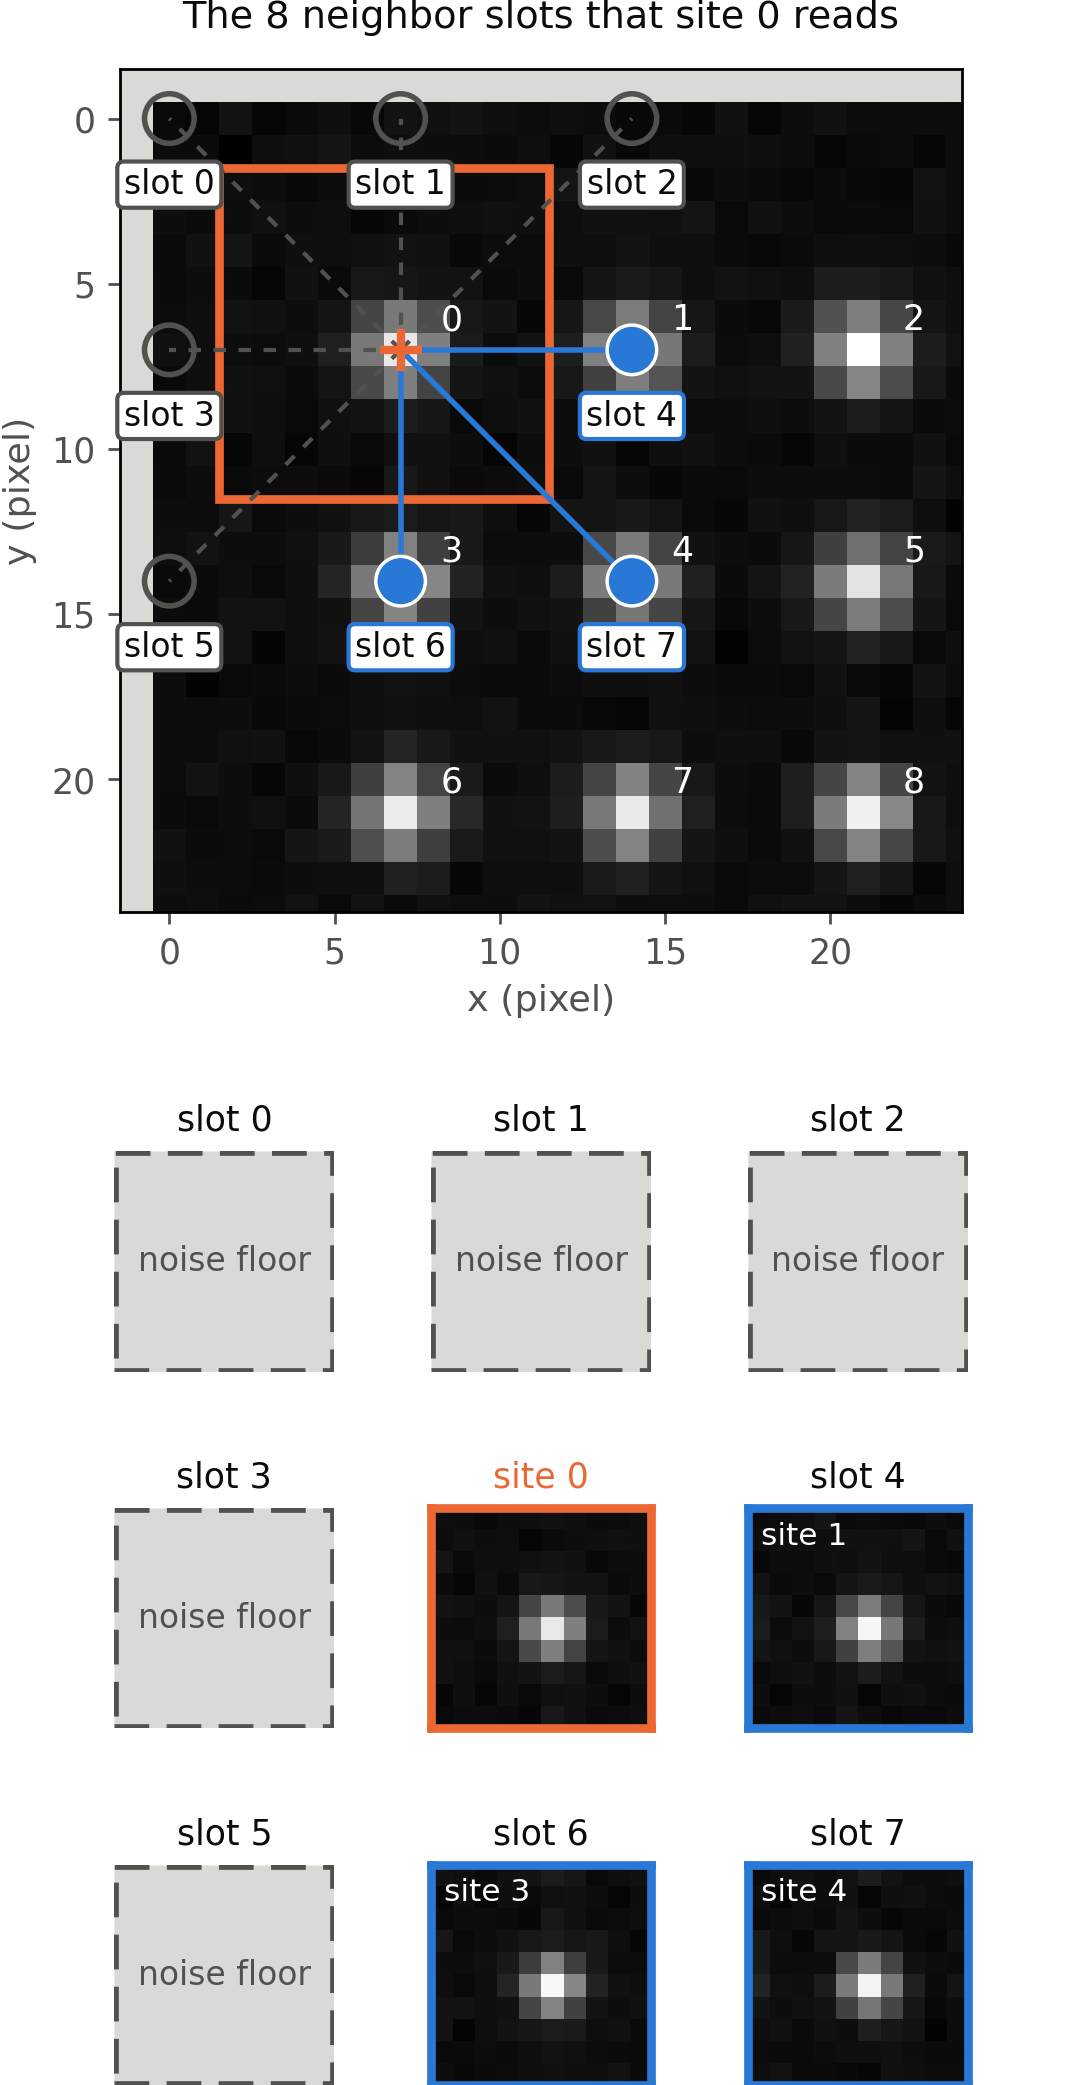
\includegraphics[width=\textwidth,height=0.8\textheight,keepaspectratio]{neighbor_table_site_0.png}
    \caption[Neighbor slots of the corner site~0 (average training image, \SI{10}{\milli\second} exposure).]{Neighbor slots of the corner site~0 (average training image, \SI{10}{\milli\second} exposure). The five slots outside the grid (dashed) are filled with the mean value of an empty site.}
    \label{fig:neighbor-slots}
\end{figure}

\section{Preprocessing Controller}\label{app:preprocessing-controller}

\begin{figure}[H]
    \centering
    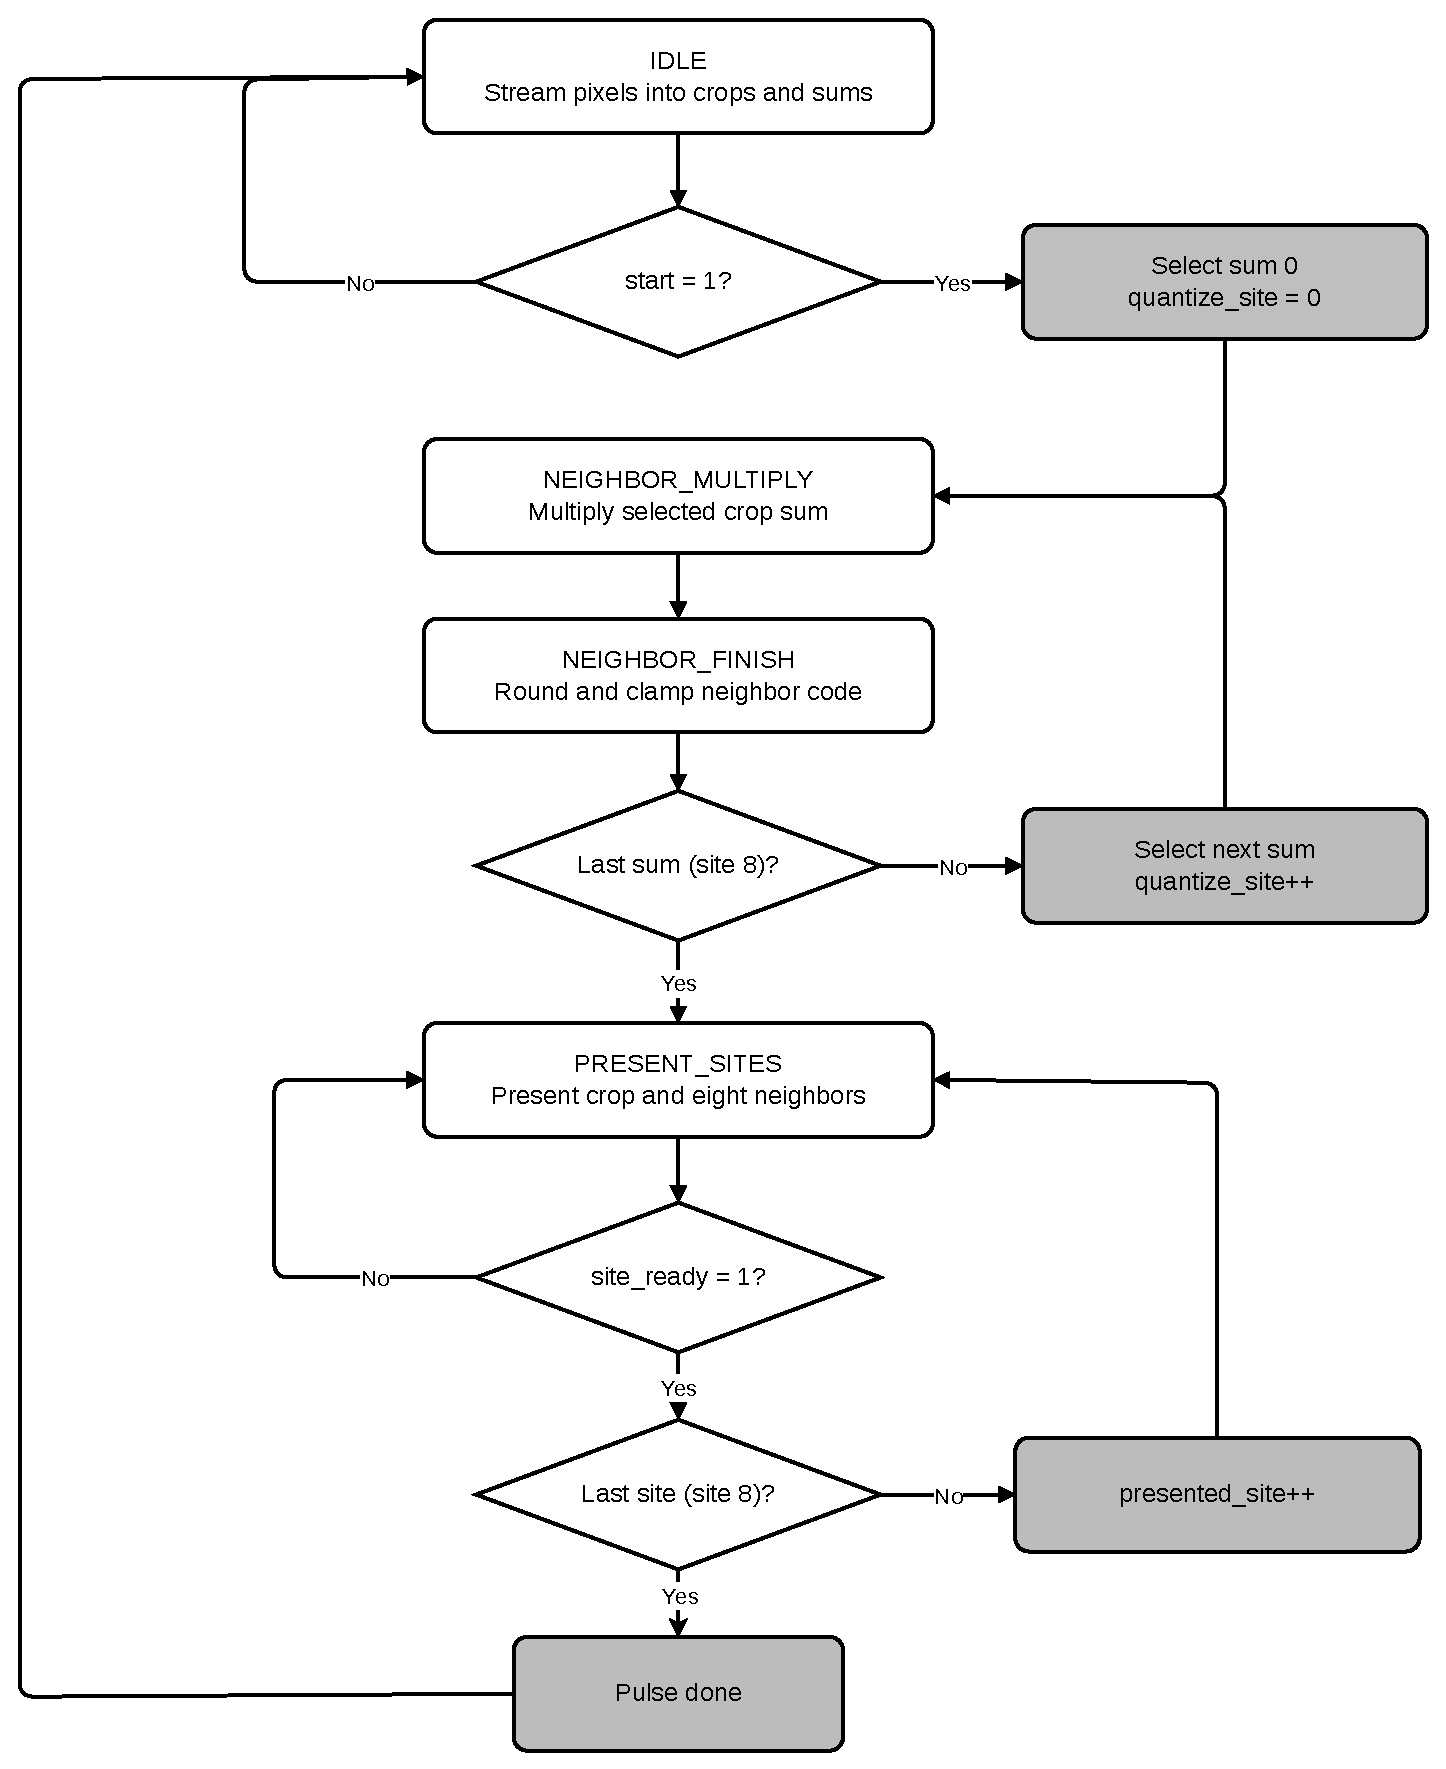
\includegraphics[width=\textwidth,height=0.82\textheight,keepaspectratio]{preprocessing_controller_cropped.pdf}
    \caption[Flowchart of the preprocessing controller.]{Flowchart of the preprocessing controller. Grey boxes indicate actions, while white boxes represent states.}
    \label{fig:preprocessing-controller}
\end{figure}

\section{Site Scheduler}\label{app:site-scheduler}

\begin{figure}[H]
    \centering
    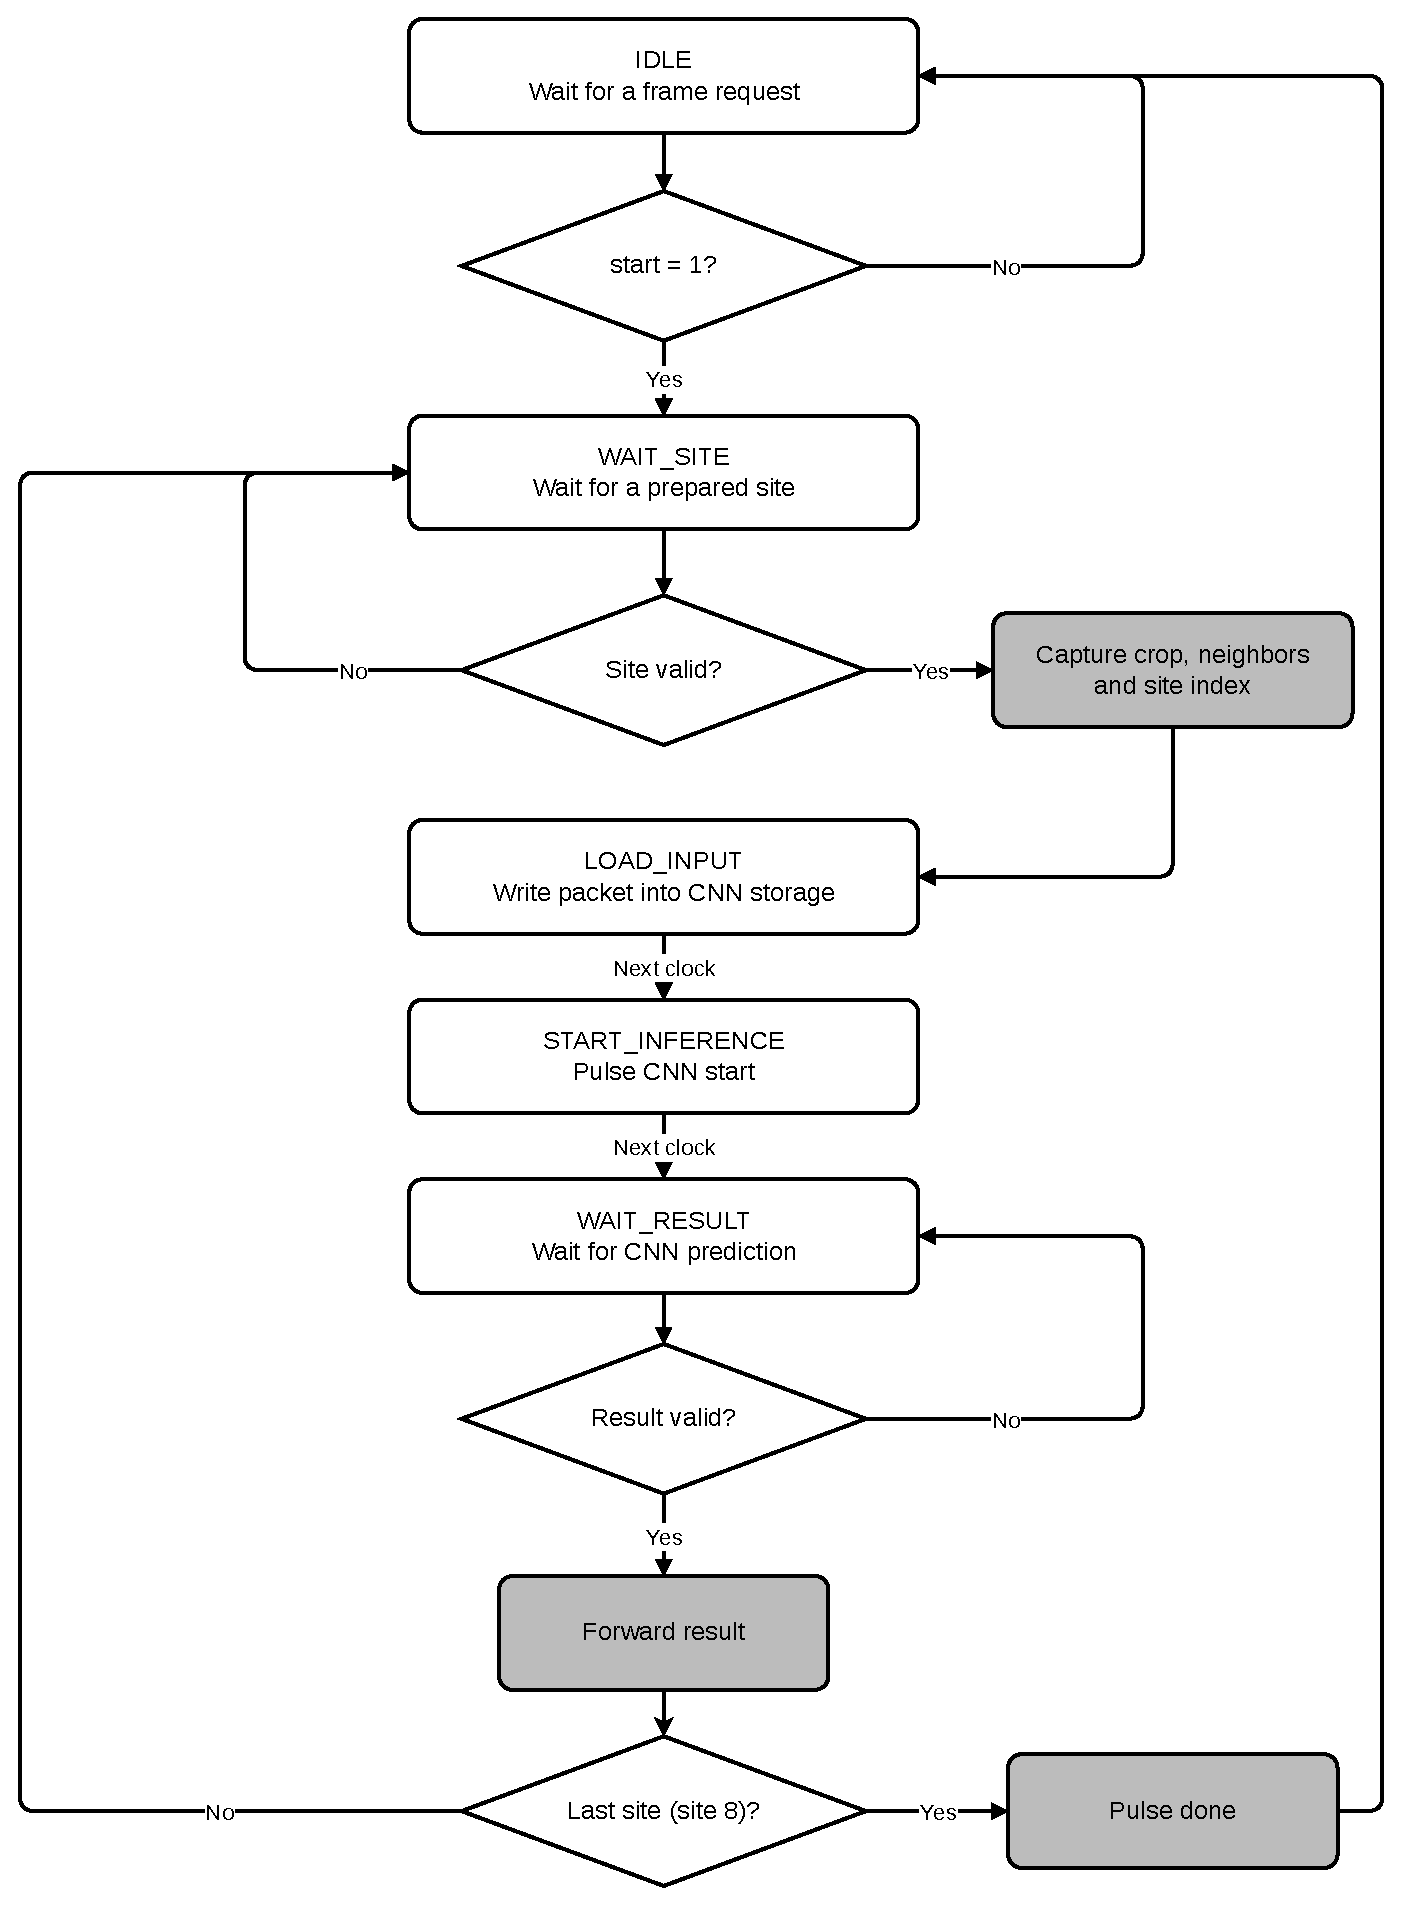
\includegraphics[width=\textwidth,height=0.85\textheight,keepaspectratio]{site_scheduler_cropped.pdf}
    \caption[Flowchart of the site scheduler.]{Flowchart of the site scheduler. Grey boxes indicate actions, while white boxes represent states.}
    \label{fig:site-scheduler}
\end{figure}

\section{CNN Controller}\label{app:cnn-controller}

\begin{figure}[H]
    \centering
    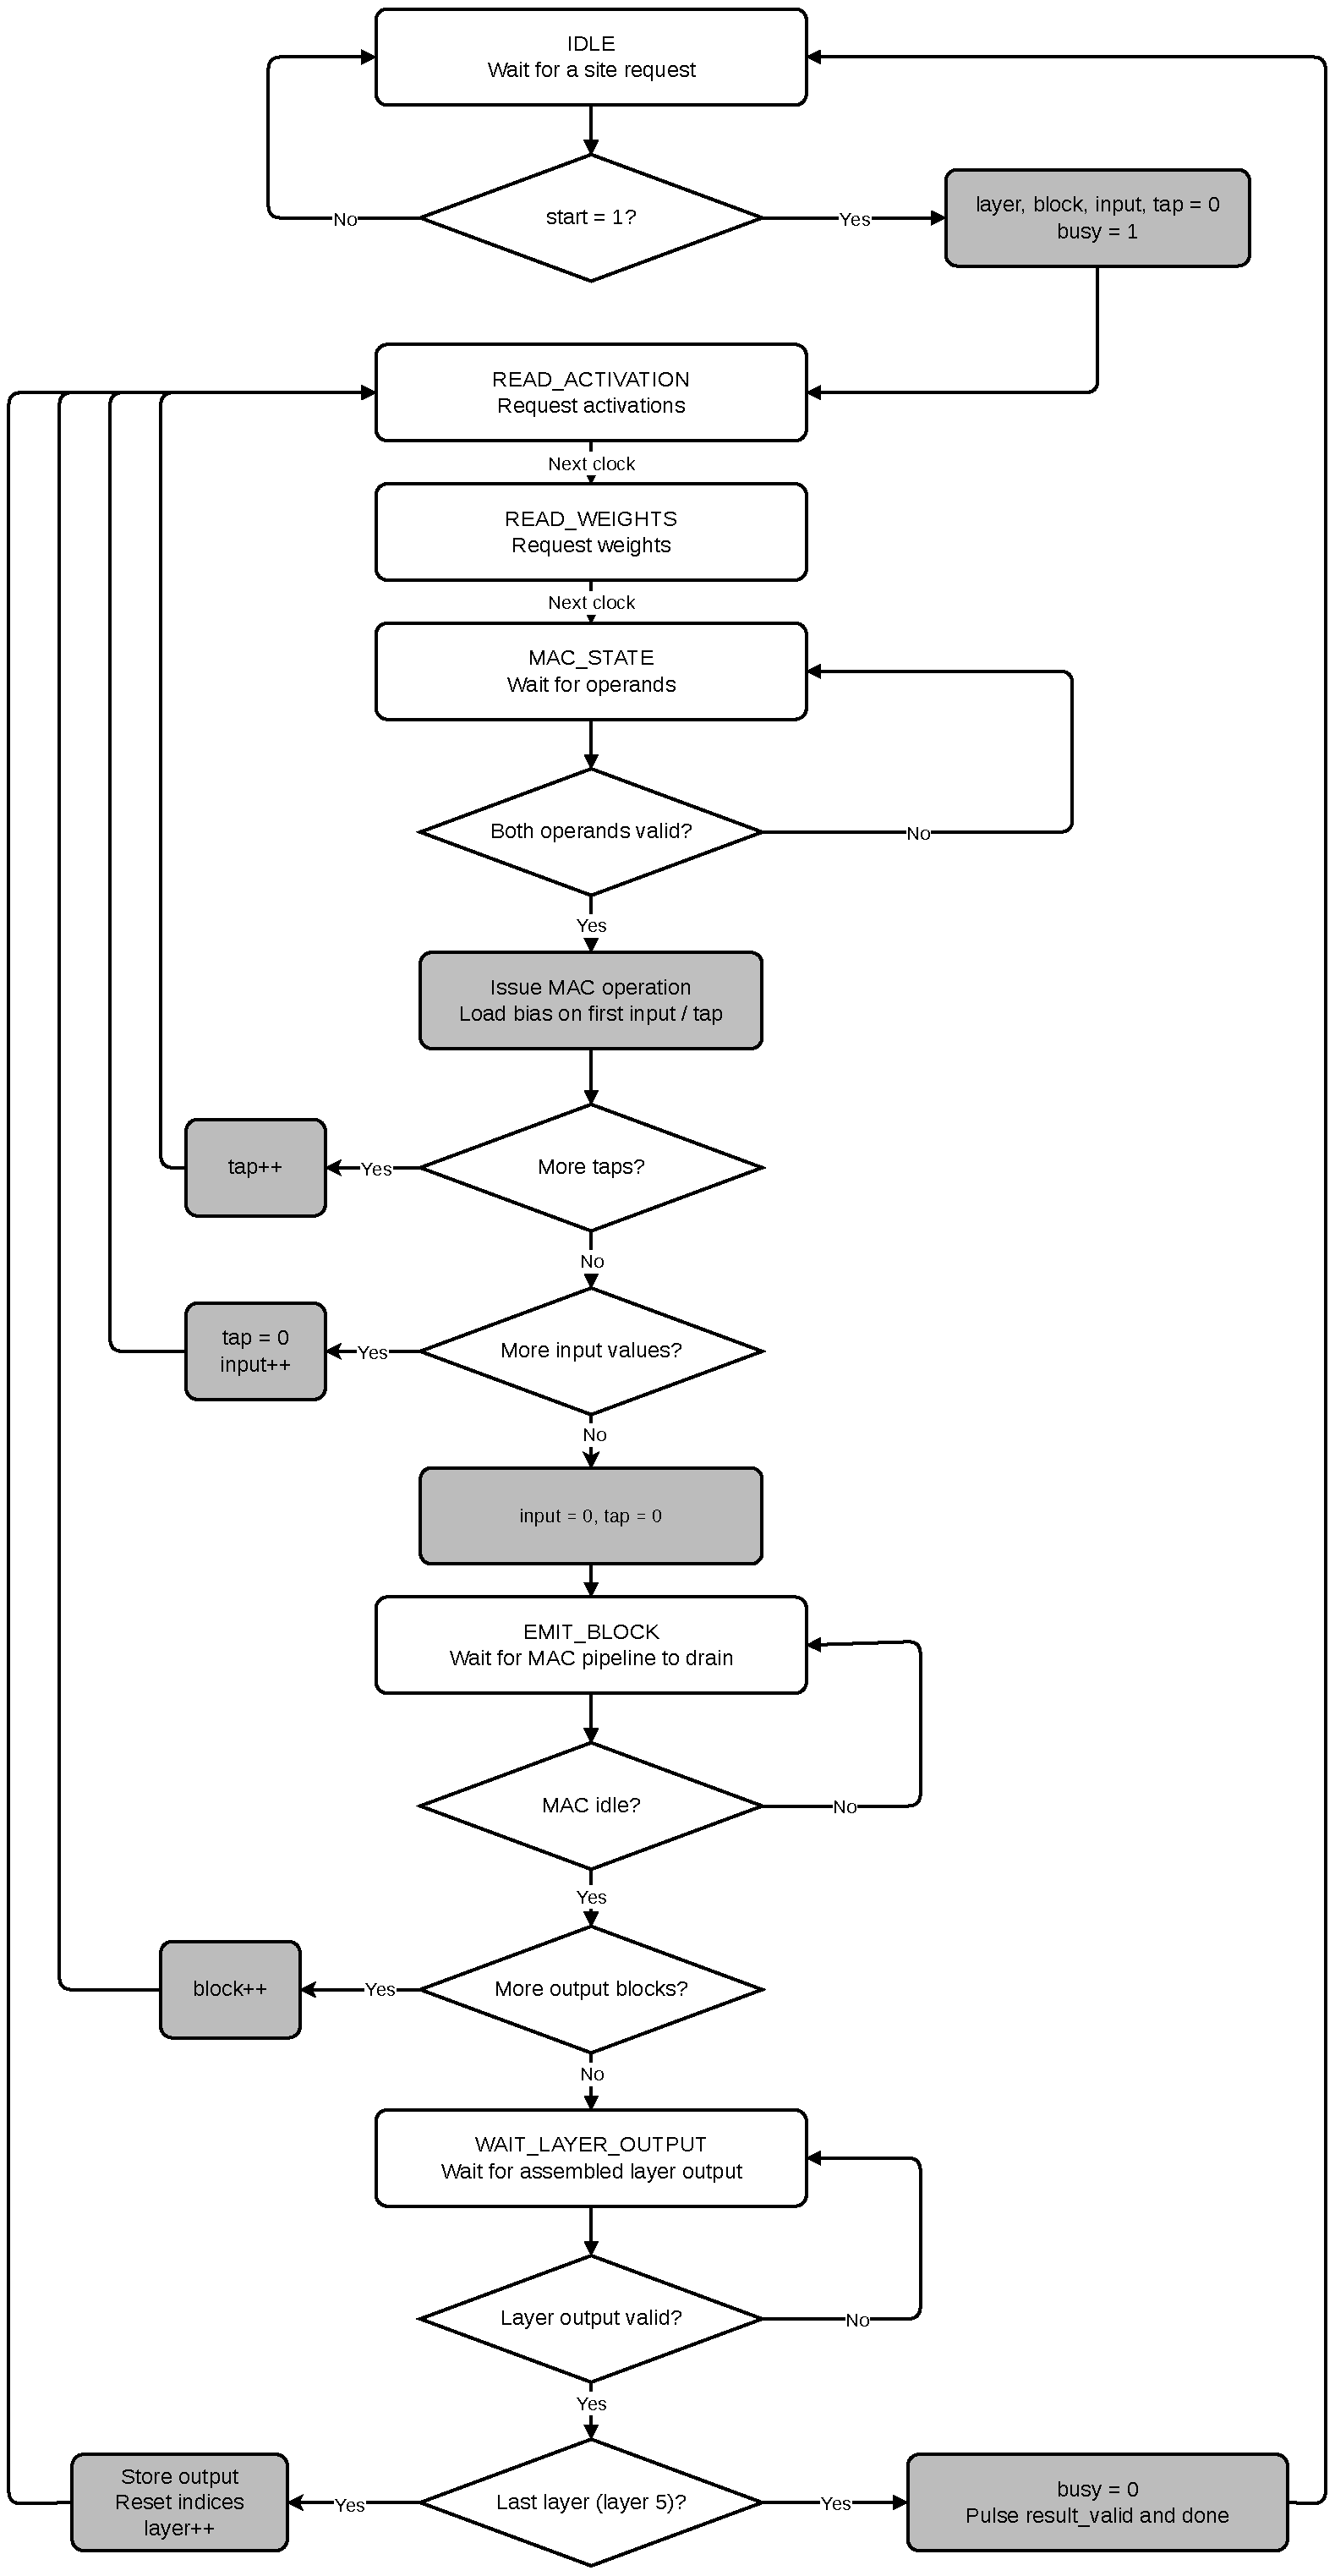
\includegraphics[width=\textwidth,height=0.85\textheight,keepaspectratio]{cnn_controller_cropped.pdf}
    \caption[Flowchart of the CNN controller.]{Flowchart of the CNN controller. Grey boxes indicate actions, while white boxes represent states.}
    \label{fig:cnn-controller}
\end{figure}


\end{document}
